\documentclass[11pt,a4paper]{article}

% Image mode: pdf.
% Image paths stay relative. In PDF mode, place same-basename PDF conversions
% of the chapter SVG files in the assets/ directory beside this source.

\usepackage{iftex}
\ifPDFTeX
  \PackageError{handout}{This template requires XeTeX or Tectonic}{Compile with xelatex or tectonic.}
\fi

\usepackage[a4paper,top=18mm,bottom=20mm,left=20mm,right=20mm,headsep=6mm]{geometry}
\usepackage{fontspec}
\usepackage{xeCJK}
\usepackage{amsmath}
\usepackage{unicode-math}

% Font settings are intentionally visible in the generated .tex file.
% These defaults target the macOS machine used for the released PDF.
% Change the family names when compiling on another system.
\setmainfont{Songti TC}
\setsansfont{Heiti TC}
\setmonofont{Menlo}
\setCJKmainfont{Songti TC}
\setCJKsansfont{Heiti TC}
\setCJKmonofont{Heiti TC}
\setmathfont{STIX Two Math}
\XeTeXlinebreaklocale "zh"
\XeTeXlinebreakskip=0pt plus 1pt

\usepackage{xcolor}
\definecolor{HandoutBlue}{HTML}{215A91}
\definecolor{HandoutBlueLight}{HTML}{EEF5FC}
\definecolor{HandoutGreen}{HTML}{39715A}
\definecolor{HandoutGreenLight}{HTML}{EFF8F3}
\definecolor{HandoutGold}{HTML}{8A641C}
\definecolor{HandoutGoldLight}{HTML}{FFF8E8}
\definecolor{HandoutInk}{HTML}{253142}
\definecolor{HandoutMuted}{HTML}{667085}

\usepackage{graphicx}
\makeatletter
% Pandoc 3 emits an accessibility `alt` key for raster/PDF images. Older
% graphicx releases do not know that key, so accept it without changing layout.
\@ifundefined{KV@Gin@alt}{\define@key{Gin}{alt}{}}{}
\newsavebox\pandoc@box
\newcommand*\pandocbounded[1]{%
  \sbox\pandoc@box{#1}%
  \Gscale@div\@tempa{\textheight}{\dimexpr\ht\pandoc@box+\dp\pandoc@box\relax}%
  \Gscale@div\@tempb{\linewidth}{\wd\pandoc@box}%
  \ifdim\@tempb\p@<\@tempa\p@\let\@tempa\@tempb\fi
  \ifdim\@tempa\p@<\p@\scalebox{\@tempa}{\usebox\pandoc@box}%
  \else\usebox{\pandoc@box}%
  \fi
}
\makeatother
\usepackage{float}
\floatplacement{figure}{H}
% Pandoc uses LTcaptype=none for uncaptioned longtables. The caption package
% expects that name to exist as a counter even though it is never displayed.
\newcounter{none}
\usepackage{caption}
\captionsetup[figure]{labelformat=empty,labelsep=none,font=small}

\usepackage{booktabs,longtable,array,calc}
\usepackage{etoolbox}
\makeatletter
\patchcmd\longtable{\par}{\if@noskipsec\mbox{}\fi\par}{}{}
\makeatother

\usepackage[most]{tcolorbox}
\tcbuselibrary{breakable,skins}
\newtcolorbox{HandoutLearningMap}{
  enhanced,breakable,colback=HandoutBlueLight,colframe=HandoutBlue,
  boxrule=0.8pt,arc=1.5mm,left=3mm,right=3mm,top=2mm,bottom=2mm,
  before skip=8pt,after skip=10pt
}
\newtcolorbox{HandoutWorkedExample}{
  enhanced,breakable,colback=HandoutGreenLight,colframe=HandoutGreen,
  boxrule=0.65pt,arc=1.5mm,left=3mm,right=3mm,top=2mm,bottom=2mm,
  before skip=8pt,after skip=10pt
}
\newtcolorbox{HandoutSelfCheck}{
  enhanced,breakable,colback=HandoutGoldLight,colframe=HandoutGold,
  boxrule=0.65pt,arc=1.5mm,left=3mm,right=3mm,top=2mm,bottom=2mm,
  before skip=8pt,after skip=10pt
}

\usepackage{titlesec}
\titleformat{\section}{\sffamily\bfseries\Large\color{HandoutBlue}}{}{0pt}{}
\titleformat{\subsection}{\sffamily\bfseries\large\color{HandoutInk}}{}{0pt}{}
\titleformat{\subsubsection}{\sffamily\bfseries\normalsize\color{HandoutInk}}{}{0pt}{}
\titlespacing*{\section}{0pt}{1.4em}{0.55em}
\titlespacing*{\subsection}{0pt}{1.15em}{0.45em}
\titlespacing*{\subsubsection}{0pt}{0.9em}{0.35em}
\setcounter{secnumdepth}{-\maxdimen}

\usepackage{hyperref}
\usepackage{bookmark}
\IfFileExists{xurl.sty}{\usepackage{xurl}}{}
\urlstyle{same}
\hypersetup{
  colorlinks=true,
  linkcolor=HandoutBlue,
  urlcolor=HandoutBlue,
  citecolor=HandoutBlue,
  pdftitle={選化III-1 化學平衡},
  pdfsubject={化學},
  pdfcreator={Pandoc with the HighSchooContent LaTeX template}
}

\setlength{\parindent}{0pt}
\setlength{\parskip}{0.55em plus 0.15em minus 0.1em}
\setlength{\emergencystretch}{3em}
\setlength{\LTpre}{0.5em}
\setlength{\LTpost}{0.5em}
\renewcommand{\arraystretch}{1.18}
\providecommand{\tightlist}{%
  \setlength{\itemsep}{0pt}\setlength{\parskip}{0pt}}
\pagestyle{plain}


\begin{document}

\begin{tcolorbox}[
  enhanced,colback=white,colframe=HandoutBlue,boxrule=1.1pt,arc=2mm,
  borderline west={3pt}{0pt}{HandoutBlue},left=5mm,right=4mm,top=4mm,bottom=4mm
]
{\sffamily\small\bfseries\color{HandoutBlue}學生講義}\par
{\sffamily\bfseries\LARGE\color{HandoutInk}選化III-1 化學平衡}\par
\vspace{0.35em}{\large 由正、逆反應速率與反應商，預測平衡組成如何受濃度、壓力、溫度與溶解條件控制}\par
\vspace{0.45em}{\small\color{HandoutMuted}%
科目：化學
\quad 課程：普通高中選修化學 III
\quad 版本：學生版｜核心＋理解
\quad 校訂：2026-08-29
}\par
\vspace{0.25em}{\small\color{HandoutMuted}範圍：現行選修化學 III 第一章主線；涵蓋動態平衡、Kc／Kp、Q 與 ICE、勒沙特列原理、Ksp／同離子效應、沉澱分離與兩項平衡實驗}\par
\end{tcolorbox}


可逆反應通常不會把反應物全部耗盡，而是在正、逆反應同時進行時形成穩定組成。平衡常數把這個組成寫成定量關係；反應商則把任一時刻的組成代入同一形式，立即給出淨反應方向。這套方法能解釋合成氨的操作條件、血液攜氧、藥物與礦物的溶解、廢水沉澱處理，也能把顏色、壓力與吸光度轉成平衡證據。

\begin{HandoutLearningMap}

\subsection{本章問題與能力}\label{ux672cux7ae0ux554fux984cux8207ux80fdux529b}

\begin{enumerate}
\def\labelenumi{\arabic{enumi}.}
\tightlist
\item
  如何用正、逆反應速率說明動態平衡，並由可測量資料判斷平衡狀態？
\item
  如何正確寫出 \(K_c\)、\(K_p\)，處理反應式反向、倍乘、相加及異相平衡？
\item
  如何用 \(Q\) 與 \(K\) 判斷方向，再以 ICE 表求平衡組成？
\item
  濃度、體積、壓力、惰性氣體、溫度與催化劑各先改變哪個量？
\item
  如何由 \(K_{sp}\) 求莫耳溶解度、判斷沉澱並設計離子分離？
\item
  如何把 NO\(_2\)/N\(_2\)O\(_4\) 與 FeSCN\(^{2+}\) 實驗寫成觀察、證據、推論與模型限制？
\end{enumerate}

\end{HandoutLearningMap}

\section{1. 可逆化學反應與化學平衡}\label{ux53efux9006ux5316ux5b78ux53cdux61c9ux8207ux5316ux5b78ux5e73ux8861}

\subsection{1.1 可逆反應與封閉系統}\label{ux53efux9006ux53cdux61c9ux8207ux5c01ux9589ux7cfbux7d71}

在相同條件下，反應物可生成產物，產物也可重新生成反應物，稱為\textbf{可逆反應}。一般寫成

\[
aA+bB\rightleftharpoons cC+dD.
\]

正向箭頭對應正反應，逆向箭頭對應逆反應。要讓生成物保留並參與逆反應，系統通常需封閉；若氣體持續逸出、沉澱被立即濾除或產物連續抽走，組成便由物質流動與反應共同決定。

\subsection{1.2 動態平衡的微觀與巨觀描述}\label{ux52d5ux614bux5e73ux8861ux7684ux5faeux89c0ux8207ux5de8ux89c0ux63cfux8ff0}

在封閉、定溫條件下，當正反應速率等於逆反應速率時，系統達到\textbf{化學平衡}：

\[
v_{\mathrm f}=v_{\mathrm r}.
\]

此時微觀上正、逆反應持續發生，兩方向單位時間的反應進度相等；巨觀上各物種濃度、分壓、顏色等與組成直接相關的量維持定值。平衡濃度不必相等；相等的是正、逆反應速率。

\begin{figure}
\centering
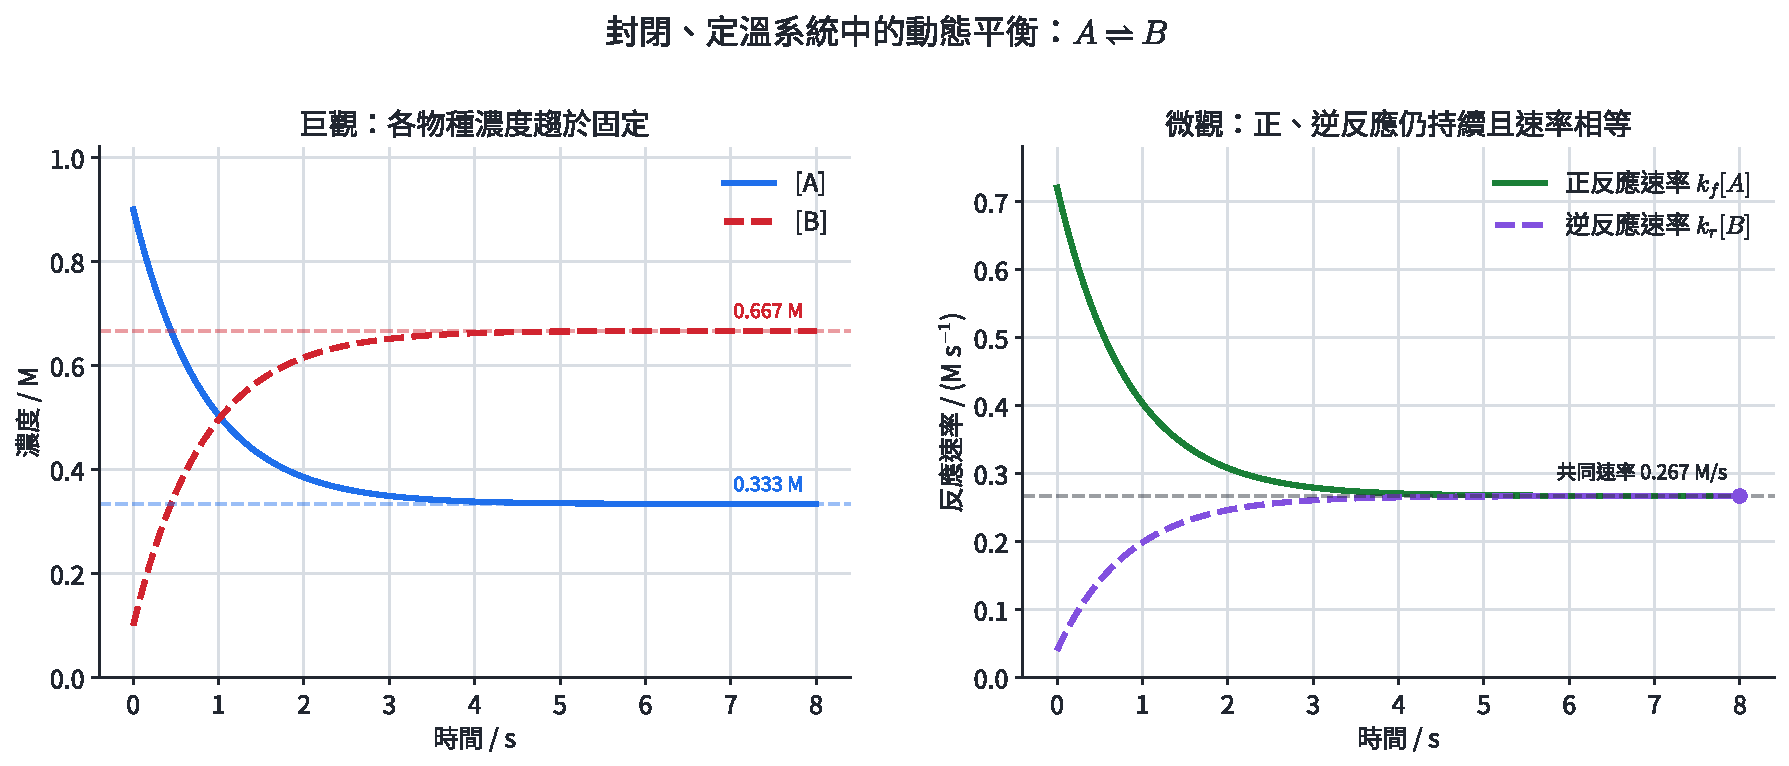
\includegraphics[width=0.98\linewidth,height=\textheight,keepaspectratio,alt={圖 1｜左圖追蹤 A、B 濃度，右圖追蹤正、逆速率；平衡判準是速率相等，而各物種濃度各自停在固定值。}]{assets/選化III-1-動態平衡濃度與速率.pdf}
\caption{圖 1｜左圖追蹤 A、B 濃度，右圖追蹤正、逆速率；平衡判準是速率相等，而各物種濃度各自停在固定值。}
\end{figure}

判斷一項巨觀量是否足以證明平衡，需確認它會隨反應進度改變。例如 \(H_2(g)+I_2(g)\rightleftharpoons2HI(g)\) 的氣體總莫耳數前後相同，定溫定容時總壓可一直不變；各物種分壓維持定值才直接對應組成固定。

\begin{HandoutWorkedExample}

\subsection{示範 1｜用正、逆速率判斷平衡}\label{ux793aux7bc4-1ux7528ux6b63ux9006ux901fux7387ux5224ux65b7ux5e73ux8861}

\(A\rightleftharpoons B\) 在某溫度下有 \(k_f=0.60\ \mathrm{s^{-1}}\)、\(k_r=0.20\ \mathrm{s^{-1}}\)。某時刻 \([A]=0.25\ \mathrm M\)、\([B]=0.75\ \mathrm M\)。

\[
v_f=k_f[A]=(0.60)(0.25)=0.150\ \mathrm{M\,s^{-1}},
\]

\[
v_r=k_r[B]=(0.20)(0.75)=0.150\ \mathrm{M\,s^{-1}}.
\]

兩速率相等，因此此組成是平衡組成。此時 \([A]\ne[B]\)，再次顯示平衡判準是兩方向速率相等。

\end{HandoutWorkedExample}

\begin{HandoutWorkedExample}

\subsection{示範 2｜選擇能辨認平衡的觀測量}\label{ux793aux7bc4-2ux9078ux64c7ux80fdux8fa8ux8a8dux5e73ux8861ux7684ux89c0ux6e2cux91cf}

對 \(N_2(g)+3H_2(g)\rightleftharpoons2NH_3(g)\)，在定溫定容密閉容器中連續量測總質量、總壓、\(NH_3\) 分壓。

密閉容器的總質量由質量守恆固定，反應開始前後都不變，因此辨識力為零。此反應氣體係數總和由 \(4\) 變成 \(2\)，反應進行會改變總莫耳數，所以總壓進入平台可作巨觀證據。\(NH_3\) 分壓直接反映其物質量，進入平台也可作證據。結論需附帶溫度、體積固定、容器無洩漏，且量測時間足以排除短暫波動。

\end{HandoutWorkedExample}

\subsection{\texorpdfstring{1.3 NO\(_2\)/N\(_2\)O\(_4\)：用顏色看見平衡移動}{1.3 NO\_2/N\_2O\_4：用顏色看見平衡移動}}\label{no_2n_2o_4ux7528ux984fux8272ux770bux898bux5e73ux8861ux79fbux52d5}

\[
2NO_2(g)\rightleftharpoons N_2O_4(g)+\text{熱}.
\]

\(NO_2\) 呈紅棕色，\(N_2O_4\) 顏色很淡。壓縮密閉注射筒時，所有氣體濃度先同時升高，所以顏色立即變深；接著淨反應向右，部分 \(NO_2\) 形成 \(N_2O_4\)，顏色逐漸變淡。新平衡的體積仍較小，因此最後通常仍比壓縮前深。這個「瞬間變化---後續鬆弛」次序是判讀平衡實驗的核心。

本實驗只能在有教師監督的實驗室或通風櫥中進行。\(NO_2\) 具急性吸入毒性；製備用濃硝酸具強腐蝕性與氧化性，NaOH 吸收液也具腐蝕性。操作需使用密閉裝置、護目鏡、合適手套與通風櫥。尾氣以 NaOH 吸收，吸收液依校內鹼性含氮廢液規範收集；暴露或洩漏依安全資料表與校內緊急程序處置。

\subsection{1.4 直接用途與模型限制}\label{ux76f4ux63a5ux7528ux9014ux8207ux6a21ux578bux9650ux5236}

血紅素與氧的結合、氣體感測器的可逆吸附、可充電電池的電極反應與工業循環製程，都需要區分「反應能否進行」與「最後停在哪個組成」。本節的動態模型描述封閉系統在指定條件下的穩定組成；活細胞與連續工廠常有物質流入、流出，屬開放穩態，需再加入流量與能量收支。

\subsection{練習 1}\label{ux7df4ux7fd2-1}

\begin{enumerate}
\def\labelenumi{\arabic{enumi}.}
\tightlist
\item
  \(A(g)\rightleftharpoons B(g)\) 在某時刻 \(v_f=2.4\times10^{-3}\)、\(v_r=1.9\times10^{-3}\ \mathrm{M\,s^{-1}}\)。寫出淨反應方向；兩速率之後如何變化才會達平衡？
\item
  對 \(2SO_2(g)+O_2(g)\rightleftharpoons2SO_3(g)\)，列出兩項可在定溫定容下反映組成固定的巨觀量。
\item
  對 \(H_2(g)+Cl_2(g)\rightleftharpoons2HCl(g)\)，說明總壓維持定值為何不足以單獨證明平衡。
\item
  平衡時每秒有 \(4.0\times10^{18}\) 個 A 分子轉成 B。每秒應有多少個 B 分子轉回 A？8 秒內兩方向各轉換多少個分子？
\item
  壓縮已達平衡的 \(NO_2/N_2O_4\) 混合氣。將「壓縮前、壓縮瞬間、新平衡」的顏色依深淺排序，並說明原因。
\end{enumerate}

\subsection{練習 1 解析}\label{ux7df4ux7fd2-1-ux89e3ux6790}

\begin{enumerate}
\def\labelenumi{\arabic{enumi}.}
\tightlist
\item
  \(v_f>v_r\)，淨反應向右。A 被淨消耗使正反應速率下降，B 淨增加使逆反應速率上升，直到 \(v_f=v_r\)。
\item
  可量測各物種濃度或分壓，例如 \(SO_2\) 分壓與 \(SO_3\) 分壓；也可量測與組成經校正連結的吸光度。
\item
  反應前後氣體係數總和都是 \(2\)。組成改變時，總莫耳數與總壓仍可保持不變。
\item
  動態平衡時兩方向速率相等，所以每秒也是 \(4.0\times10^{18}\) 個 B 轉回 A。8 秒內每一方向均轉換 \(3.2\times10^{19}\) 個；淨變化為零。
\item
  壓縮瞬間最深，新平衡次之，壓縮前最淡。瞬間體積減少使 \([NO_2]\) 增大；接著 \(2NO_2\to N_2O_4\) 淨進行而變淡；新平衡仍在較小體積，\(NO_2\) 濃度通常高於壓縮前。
\end{enumerate}

\section{2. 平衡常數、反應商與平衡組成}\label{ux5e73ux8861ux5e38ux6578ux53cdux61c9ux5546ux8207ux5e73ux8861ux7d44ux6210}

\subsection{\texorpdfstring{2.1 \(K_c\)、\(K_p\) 與標準狀態}{2.1 K\_c、K\_p 與標準狀態}}\label{k_ck_p-ux8207ux6a19ux6e96ux72c0ux614b}

對 \(aA(g)+bB(g)\rightleftharpoons cC(g)+dD(g)\)，

\[
K_c=\frac{[C]^c[D]^d}{[A]^a[B]^b},\qquad
K_p=\frac{(P_C)^c(P_D)^d}{(P_A)^a(P_B)^b}.
\]

嚴格熱力學定義使用相對於標準態的活性或壓力比，因此 \(K\) 無因次。高中計算常直接代入以 \(\mathrm{mol\,L^{-1}}\) 或 atm 表示的數值；同一題需使用一致單位與同一溫度。理想氣體滿足 \(P_i=[i]RT\)，所以

\[
K_p=K_c(RT)^{\Delta n_g},\qquad
\Delta n_g=(c+d)-(a+b),
\]

其中只計氣態物種係數。

\subsection{\texorpdfstring{2.2 反應式改寫與 \(K\) 的代數規則}{2.2 反應式改寫與 K 的代數規則}}\label{ux53cdux61c9ux5f0fux6539ux5bebux8207-k-ux7684ux4ee3ux6578ux898fux5247}

\begin{itemize}
\tightlist
\item
  反應反向：\(K'=1/K\)。
\item
  全部係數乘 \(n\)：\(K'=K^n\)。
\item
  多個反應式相加：總反應的 \(K\) 為各步 \(K\) 相乘。
\end{itemize}

\begin{figure}
\centering
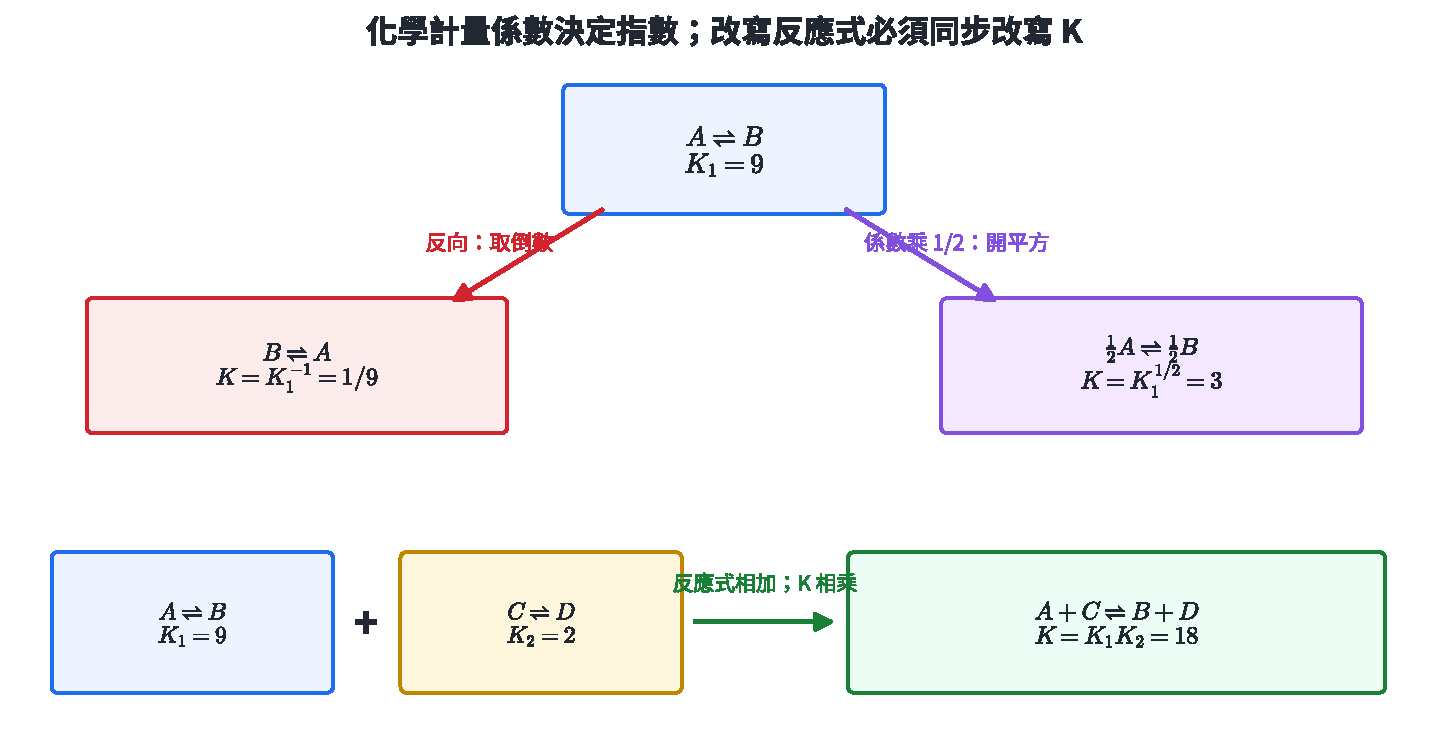
\includegraphics[width=0.96\linewidth,height=\textheight,keepaspectratio,alt={圖 2｜由 A\textbackslash rightleftharpoons B、K\_1=9 追蹤反向與係數乘二分之一；下列另把 K\_2=2 的反應相加，總反應 K=K\_1K\_2=18。}]{assets/選化III-1-反應式與平衡常數.pdf}
\caption{圖 2｜由 \(A\rightleftharpoons B\)、\(K_1=9\) 追蹤反向與係數乘二分之一；下列另把 \(K_2=2\) 的反應相加，總反應 \(K=K_1K_2=18\)。}
\end{figure}

\begin{HandoutWorkedExample}

\subsection{\texorpdfstring{示範 3｜寫出 \(K_c\)、\(K_p\) 並連結兩者}{示範 3｜寫出 K\_c、K\_p 並連結兩者}}\label{ux793aux7bc4-3ux5bebux51fa-k_ck_p-ux4e26ux9023ux7d50ux5169ux8005}

對 \(N_2(g)+3H_2(g)\rightleftharpoons2NH_3(g)\)，

\[
K_c=\frac{[NH_3]^2}{[N_2][H_2]^3},\qquad
K_p=\frac{P_{NH_3}^2}{P_{N_2}P_{H_2}^3}.
\]

\(\Delta n_g=2-(1+3)=-2\)，所以 \(K_p=K_c(RT)^{-2}=K_c/(RT)^2\)。

\end{HandoutWorkedExample}

\begin{HandoutWorkedExample}

\subsection{\texorpdfstring{示範 4｜由已知反應求改寫反應的 \(K\)}{示範 4｜由已知反應求改寫反應的 K}}\label{ux793aux7bc4-4ux7531ux5df2ux77e5ux53cdux61c9ux6c42ux6539ux5bebux53cdux61c9ux7684-k}

已知 \(2SO_2+O_2\rightleftharpoons2SO_3\) 的 \(K=4.0\times10^5\)。求 \(SO_3\rightleftharpoons SO_2+\tfrac12O_2\) 的 \(K'\)。

新反應先反向，再把係數乘 \(1/2\)：

\[
K'=\left(\frac1K\right)^{1/2}
=\frac{1}{\sqrt{4.0\times10^5}}
=1.58\times10^{-3}.
\]

\end{HandoutWorkedExample}

\subsection{\texorpdfstring{2.3 反應商 \(Q\) 與方向}{2.3 反應商 Q 與方向}}\label{ux53cdux61c9ux5546-q-ux8207ux65b9ux5411}

反應商把某一時刻的濃度或分壓代入與 \(K\) 相同的式子。固定溫度下，\(Q<K\) 時淨反應向右；\(Q=K\) 時在平衡；\(Q>K\) 時淨反應向左。

\begin{figure}
\centering
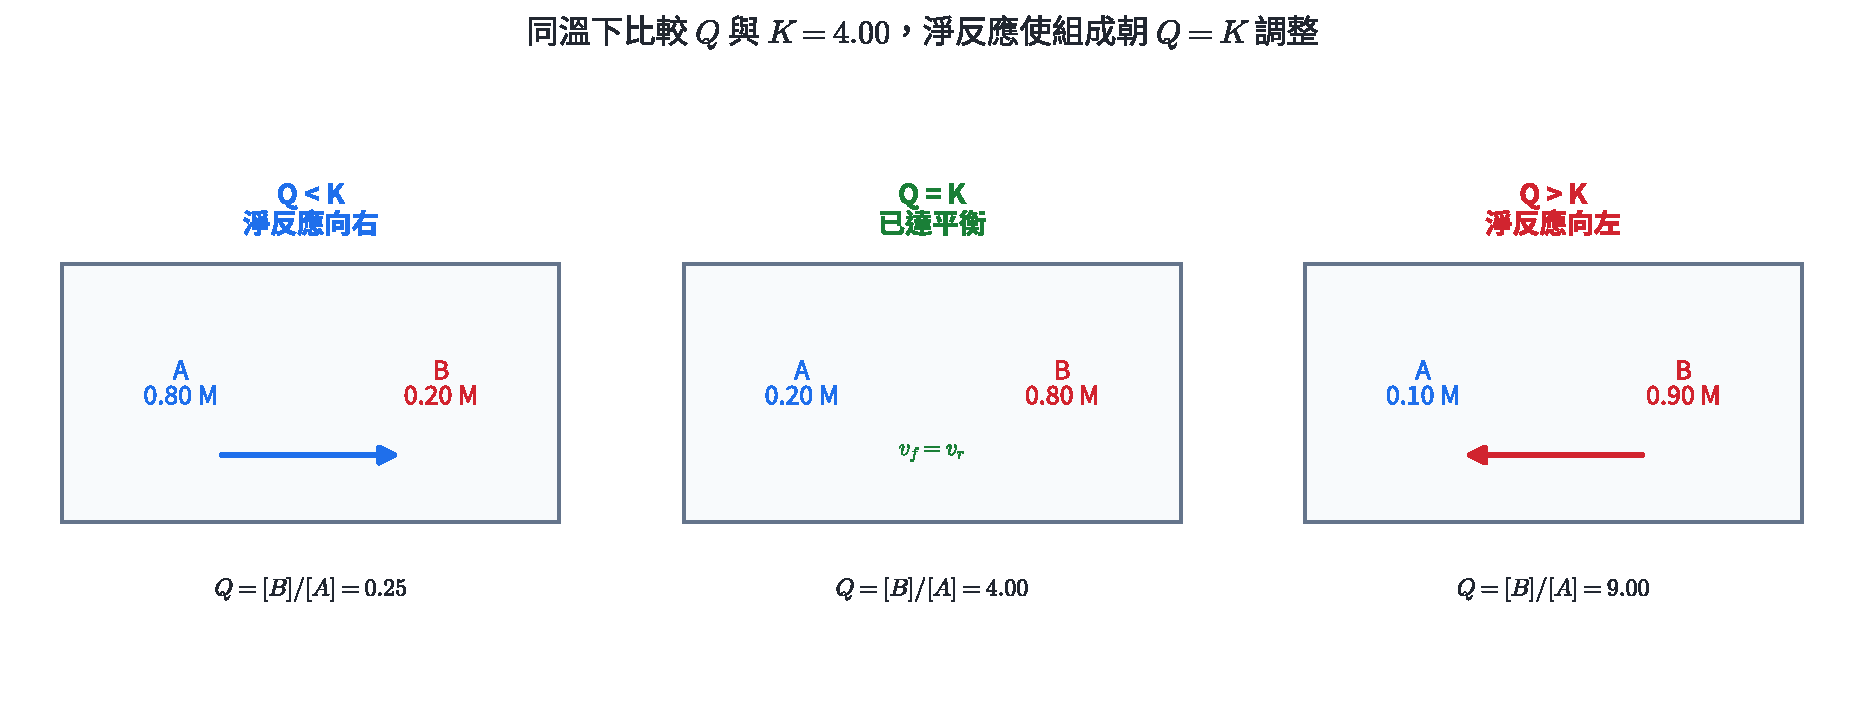
\includegraphics[width=0.95\linewidth,height=\textheight,keepaspectratio,alt={圖 3｜三個 A\textbackslash rightleftharpoons B 狀態使用同一個 K=4；箭頭方向由 Q/K 的數值關係決定。}]{assets/選化III-1-反應商判斷方向.pdf}
\caption{圖 3｜三個 \(A\rightleftharpoons B\) 狀態使用同一個 \(K=4\)；箭頭方向由 \(Q/K\) 的數值關係決定。}
\end{figure}

\begin{HandoutWorkedExample}

\subsection{\texorpdfstring{示範 5｜由 \(Q\) 判斷淨反應方向}{示範 5｜由 Q 判斷淨反應方向}}\label{ux793aux7bc4-5ux7531-q-ux5224ux65b7ux6de8ux53cdux61c9ux65b9ux5411}

\(H_2+I_2\rightleftharpoons2HI\) 的 \(K_c=50.0\)。某時刻 \([H_2]=0.20\)、\([I_2]=0.10\)、\([HI]=0.50\ \mathrm M\)。

\[
Q_c=\frac{(0.50)^2}{(0.20)(0.10)}=12.5<K_c.
\]

淨反應向右；\(H_2\)、\(I_2\) 淨減少，\(HI\) 淨增加，直到 \(Q_c\) 回到 50.0。

\end{HandoutWorkedExample}

\subsection{2.4 ICE 表與反應進度}\label{ice-ux8868ux8207ux53cdux61c9ux9032ux5ea6}

ICE 分別代表 initial、change、equilibrium。C 列由單一反應進度 \(x\) 乘化學計量係數；代入 \(K\) 後解 \(x\)，再檢查平衡濃度皆非負且回代得到原 \(K\)。

\begin{figure}
\centering
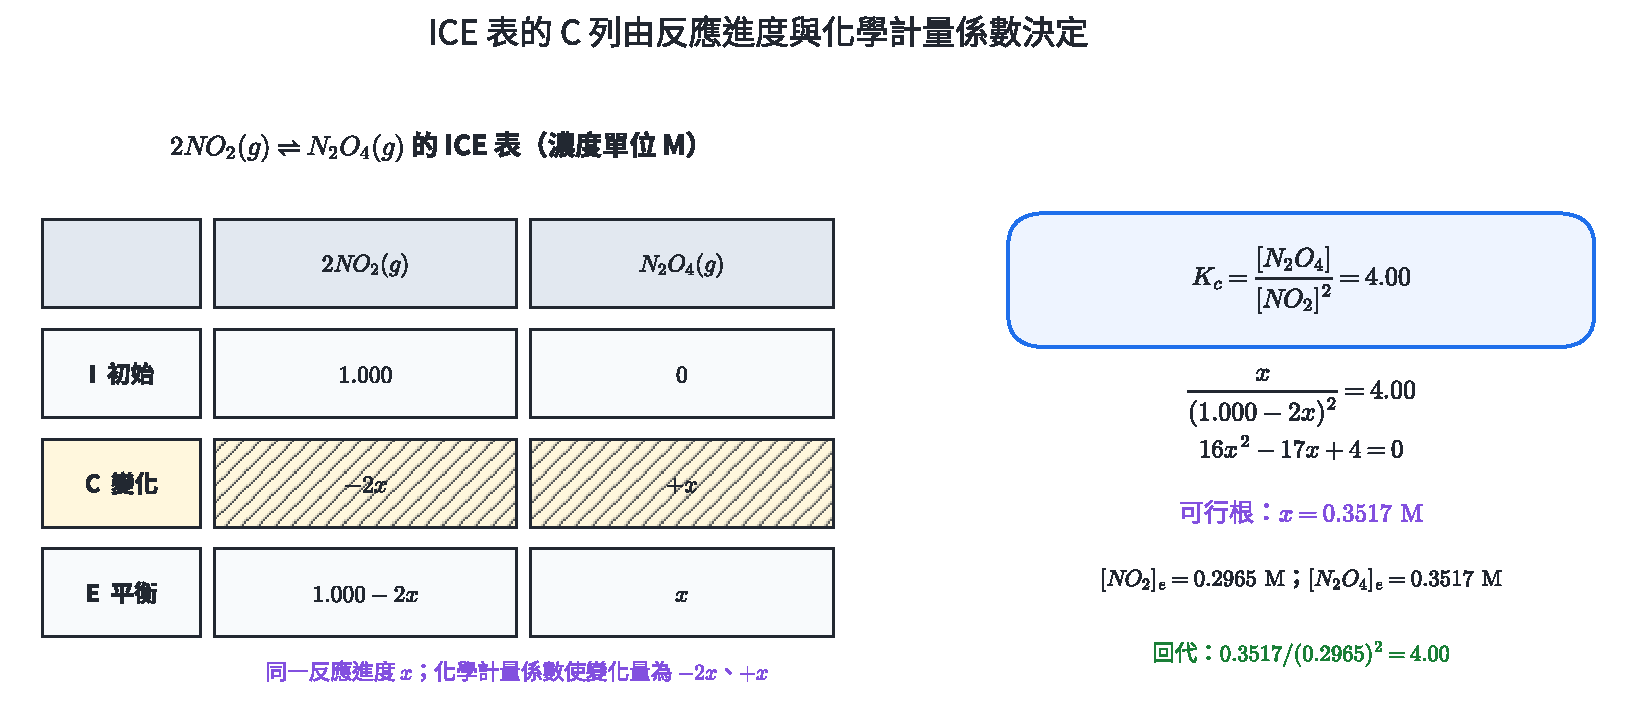
\includegraphics[width=0.96\linewidth,height=\textheight,keepaspectratio,alt={圖 4｜2\textbackslash mathrm\{NO\_2\}\textbackslash rightleftharpoons\textbackslash mathrm\{N\_2O\_4\} 的 C 列為 -2x、+x；右側用精確二次解回代 K\_c=4.00。}]{assets/選化III-1-ICE與反應進度.pdf}
\caption{圖 4｜\(2\mathrm{NO_2}\rightleftharpoons\mathrm{N_2O_4}\) 的 \(C\) 列為 \(-2x\)、\(+x\)；右側用精確二次解回代 \(K_c=4.00\)。}
\end{figure}

\begin{HandoutWorkedExample}

\subsection{示範 6｜由初始濃度求平衡組成}\label{ux793aux7bc4-6ux7531ux521dux59cbux6fc3ux5ea6ux6c42ux5e73ux8861ux7d44ux6210}

\(2NO_2\rightleftharpoons N_2O_4\) 的 \(K_c=4.00\)。初始 \([NO_2]=1.000\ \mathrm M\)、\([N_2O_4]=0\)。令生成 \(N_2O_4\) 的濃度為 \(x\)：

{\def\LTcaptype{none} % do not increment counter
\begin{longtable}[]{@{}lrr@{}}
\toprule\noalign{}
& \(NO_2\) & \(N_2O_4\) \\
\midrule\noalign{}
\endhead
\bottomrule\noalign{}
\endlastfoot
I & \(1.000\) & \(0\) \\
C & \(-2x\) & \(+x\) \\
E & \(1.000-2x\) & \(x\) \\
\end{longtable}
}

\[
4.00=\frac{x}{(1.000-2x)^2}.
\]

可行根 \(x=0.3517\ \mathrm M\)，所以 \([NO_2]_e=0.2965\ \mathrm M\)、\([N_2O_4]_e=0.3517\ \mathrm M\)。回代為 \(4.00\)。

\end{HandoutWorkedExample}

\subsection{2.5 均相與異相平衡}\label{ux5747ux76f8ux8207ux7570ux76f8ux5e73ux8861}

所有物種在同一相，稱為均相平衡；跨越兩種以上相，稱為異相平衡。純固體與純液體在固定溫壓下的活性定為 1，因此不寫入平衡式。例如

\[
CaCO_3(s)\rightleftharpoons CaO(s)+CO_2(g),\qquad K_p=P_{CO_2}.
\]

\begin{figure}
\centering
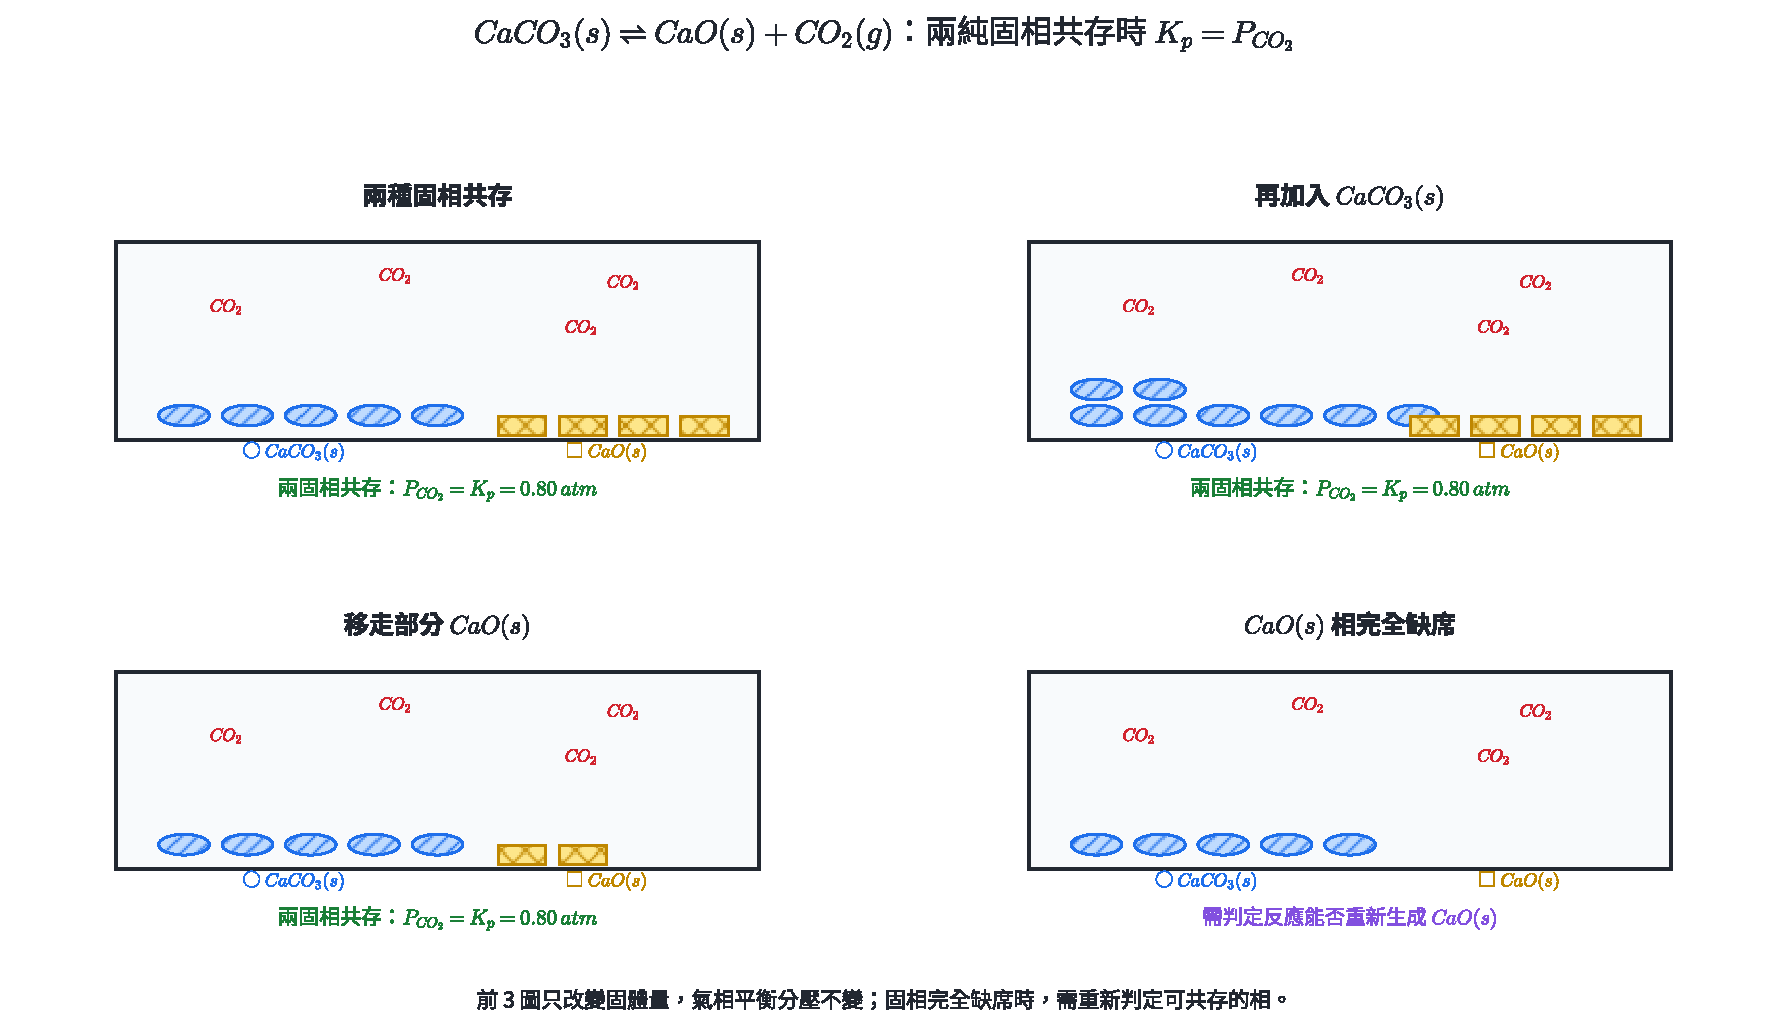
\includegraphics[width=0.96\linewidth,height=\textheight,keepaspectratio,alt={圖 5｜前三圖中 CaCO3、CaO 兩固相仍共存，改變固體量不改變平衡 CO2 分壓；第四圖顯示 CaO 相完全缺席後需重新判定可共存的相。}]{assets/選化III-1-異相平衡與活性.pdf}
\caption{圖 5｜前三圖中 CaCO3、CaO 兩固相仍共存，改變固體量不改變平衡 CO2 分壓；第四圖顯示 CaO 相完全缺席後需重新判定可共存的相。}
\end{figure}

\begin{HandoutWorkedExample}

\subsection{\texorpdfstring{示範 7｜\(K_c\) 轉成 \(K_p\)}{示範 7｜K\_c 轉成 K\_p}}\label{ux793aux7bc4-7k_c-ux8f49ux6210-k_p}

在 \(500\ \mathrm K\)，\(2SO_2+O_2\rightleftharpoons2SO_3\) 的 \(K_c=1.60\times10^3\)。取 \(R=0.082057\ \mathrm{L\,atm\,mol^{-1}\,K^{-1}}\)。\(\Delta n_g=-1\)，因此

\[
K_p=\frac{1.60\times10^3}{(0.082057)(500)}=39.0.
\]

\end{HandoutWorkedExample}

\subsection{2.6 比色量測平衡常數}\label{ux6bd4ux8272ux91cfux6e2cux5e73ux8861ux5e38ux6578}

對 \(Fe^{3+}+SCN^-\rightleftharpoons FeSCN^{2+}\)，紅色配合物的吸光度在適用濃度範圍近似滿足 \(A=\varepsilon\ell c\)。標準液以大量過量 \(Fe^{3+}\) 使 \(SCN^-\) 近似完全形成配合物，再用等吸光度與不同光徑求未知平衡濃度。

\begin{figure}
\centering
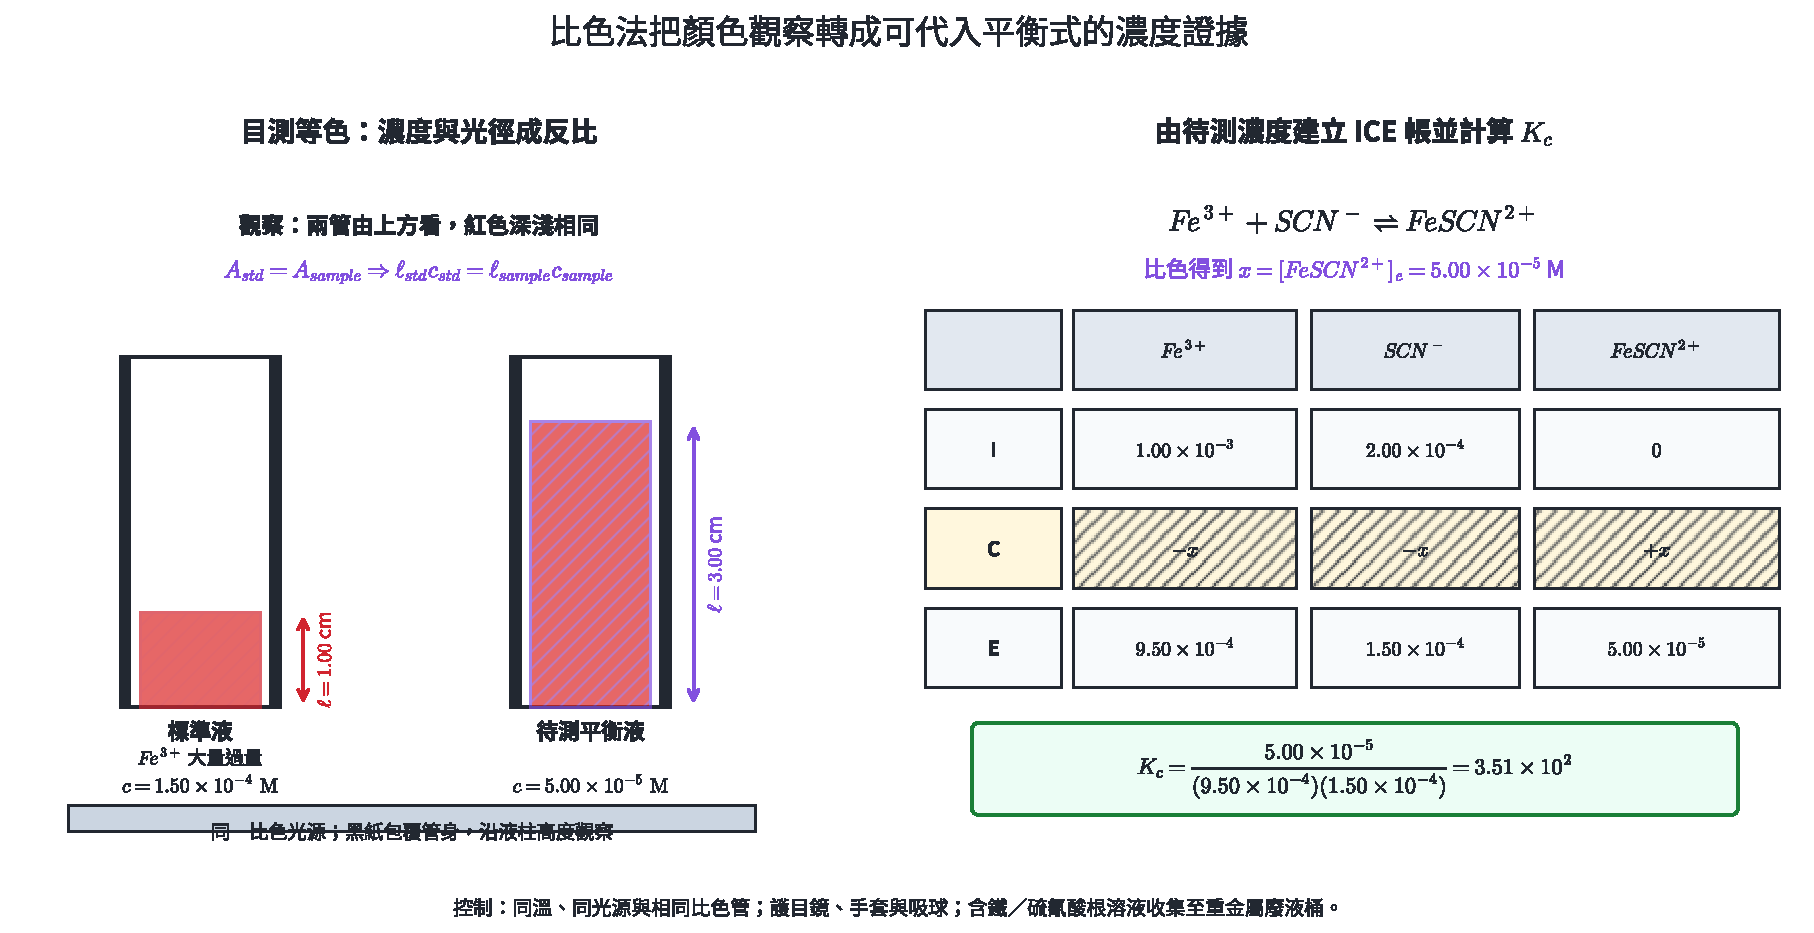
\includegraphics[width=0.99\linewidth,height=\textheight,keepaspectratio,alt={圖 6｜左圖以兩支比色管的液柱高度建立等吸光度關係，右圖把待測濃度寫入 ICE 表並計算 K\_c。}]{assets/選化III-1-FeSCN平衡常數實驗.pdf}
\caption{圖 6｜左圖以兩支比色管的液柱高度建立等吸光度關係，右圖把待測濃度寫入 ICE 表並計算 \(K_c\)。}
\end{figure}

圖 6 中 \(1.00\ \mathrm{cm}\times1.50\times10^{-4}\ \mathrm M=3.00\ \mathrm{cm}\times5.00\times10^{-5}\ \mathrm M\)，所以樣品 \([FeSCN^{2+}]_e=5.00\times10^{-5}\ \mathrm M\)；再由 ICE 得 \(K_c=3.51\times10^2\)。

實驗控制同一溫度、光源或波長、試管材質與潔淨度、觀察幾何。硝酸鐵溶液具氧化性與刺激性，酸化溶液具腐蝕性，KSCN 應避免與強酸及皮膚接觸；使用護目鏡、手套與吸球，所有含鐵與硫氰酸根溶液收集為指定無機／重金屬廢液。肉眼等色與「標準液近完全反應」是主要模型限制。

\subsection{練習 2}\label{ux7df4ux7fd2-2}

\begin{enumerate}
\def\labelenumi{\arabic{enumi}.}
\tightlist
\item
  寫出 \(CaCO_3(s)\rightleftharpoons CaO(s)+CO_2(g)\) 的 \(K_c\) 與 \(K_p\)。在兩固相皆存在時加入更多 \(CaCO_3\)，平衡 \(CO_2\) 分壓如何？
\item
  已知 \(A\rightleftharpoons2B\) 的 \(K=16\)。求 \(B\rightleftharpoons\tfrac12A\) 的 \(K'\)。
\item
  \(CO+H_2O\rightleftharpoons CO_2+H_2\) 的 \(K_c=4.0\)。某時刻四者濃度依序為 \(0.40,0.20,0.10,0.80\ \mathrm M\)，判斷方向。
\item
  \(A\rightleftharpoons2B\) 的 \(K_c=4.00\)。初始只有 \([A]=1.00\ \mathrm M\)，求平衡濃度。
\item
  \(N_2O_4\rightleftharpoons2NO_2\) 在 \(300\ \mathrm K\) 的 \(K_c=0.200\)。求 \(K_p\)，取 \(R=0.082057\)。
\item
  FeSCN\(^{2+}\) 比色中，標準液濃度 \(1.20\times10^{-4}\ \mathrm M\)、光徑 \(1.00\ \mathrm{cm}\)；未知液光徑 \(2.40\ \mathrm{cm}\) 時顏色相同。求未知液濃度。
\end{enumerate}

\subsection{練習 2 解析}\label{ux7df4ux7fd2-2-ux89e3ux6790}

\begin{enumerate}
\def\labelenumi{\arabic{enumi}.}
\tightlist
\item
  \(K_c=[CO_2]\)、\(K_p=P_{CO_2}\)。純固體活性固定；兩固相仍共存且溫度不變時，加入固體不改變 \(K\)、\(Q\) 或平衡分壓。
\item
  先反向再乘 \(1/2\)：\(K'=(1/16)^{1/2}=1/4\)。
\item
  \(Q_c=(0.10)(0.80)/[(0.40)(0.20)]=1.0<K_c\)，淨反應向右。
\item
  令 A 消耗 \(x\)，則 \([A]_e=1-x\)、\([B]_e=2x\)。由 \(4=(2x)^2/(1-x)\) 得可行根 \(x=0.618\)，所以 \([A]_e=0.382\ \mathrm M\)、\([B]_e=1.236\ \mathrm M\)。
\item
  \(\Delta n_g=1\)，\(K_p=(0.200)(0.082057)(300)=4.92\)。
\item
  \(\ell_1c_1=\ell_2c_2\)，所以 \(c_2=(1.00)(1.20\times10^{-4})/2.40=5.00\times10^{-5}\ \mathrm M\)。
\end{enumerate}

\section{3. 勒沙特列原理與條件改變}\label{ux52d2ux6c99ux7279ux5217ux539fux7406ux8207ux689dux4ef6ux6539ux8b8a}

\subsection{3.1 原理的定量版本}\label{ux539fux7406ux7684ux5b9aux91cfux7248ux672c}

勒沙特列原理指出，平衡系統受到條件改變時，會經由淨反應建立新平衡，使擾動的影響部分減弱。定量判斷依序為：寫 \(K\) 式，只改擾動瞬間直接受影響的量，算新 \(Q\)，最後依 \(Q/K\) 寫後續變化。

\begin{figure}
\centering
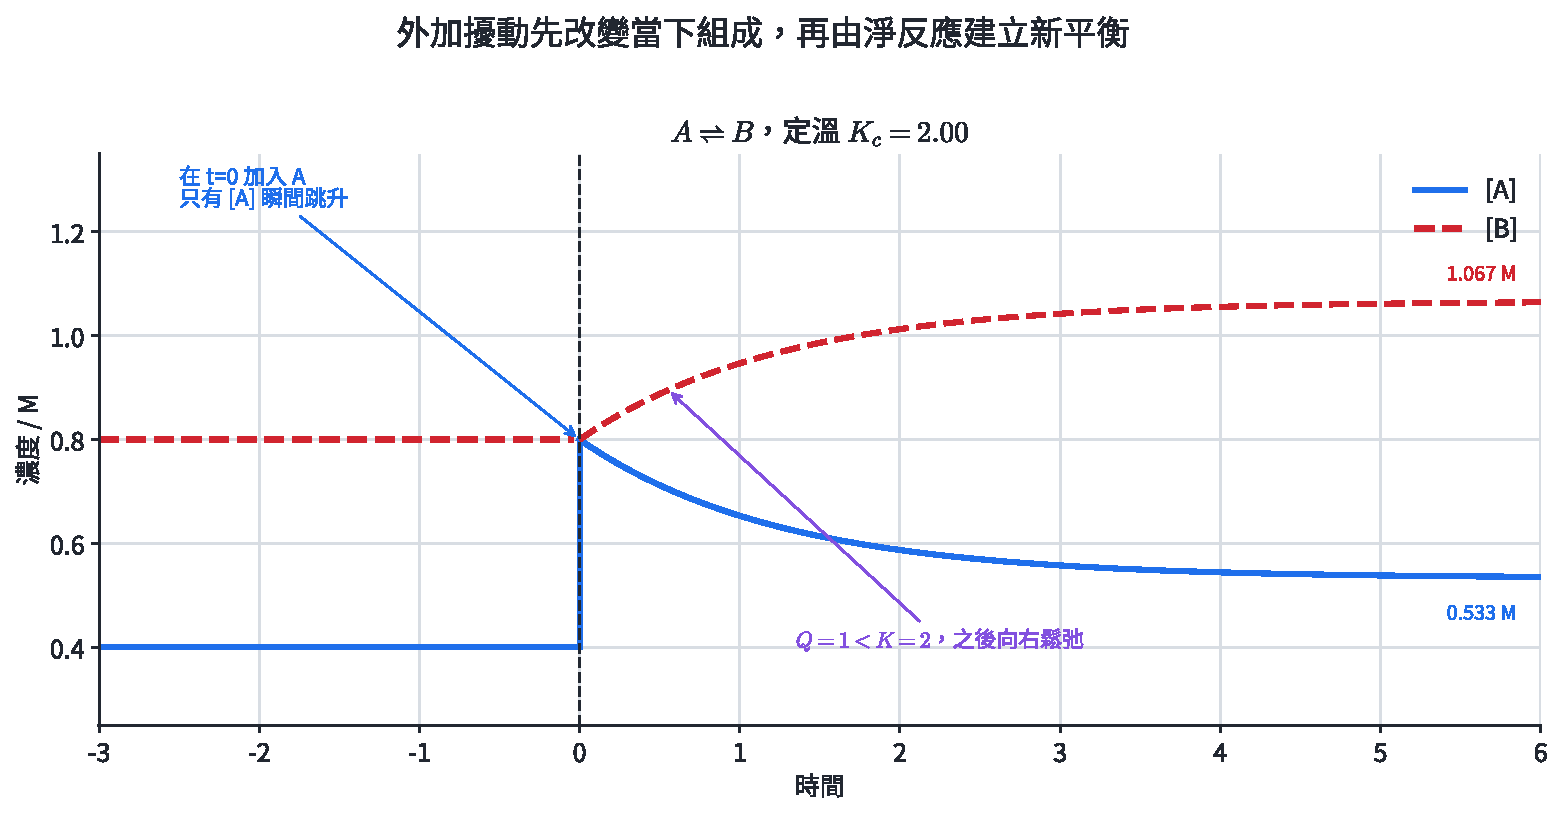
\includegraphics[width=0.96\linewidth,height=\textheight,keepaspectratio,alt={圖 7｜在 A\textbackslash rightleftharpoons B、K=2 的平衡中加入 A；只有 A 濃度瞬間跳升，Q 由 2 降為 1，之後 B 淨生成並回到 Q=2。}]{assets/選化III-1-濃度擾動的瞬間與鬆弛.pdf}
\caption{圖 7｜在 \(A\rightleftharpoons B\)、\(K=2\) 的平衡中加入 \(A\)；只有 \(A\) 濃度瞬間跳升，\(Q\) 由 \(2\) 降為 \(1\)，之後 \(B\) 淨生成並回到 \(Q=2\)。}
\end{figure}

\begin{HandoutWorkedExample}

\subsection{示範 8｜濃度擾動的瞬間與新平衡}\label{ux793aux7bc4-8ux6fc3ux5ea6ux64feux52d5ux7684ux77acux9593ux8207ux65b0ux5e73ux8861}

\(A\rightleftharpoons B\) 的 \(K_c=2.00\)，原平衡 \([A]=0.40\)、\([B]=0.80\ \mathrm M\)。瞬間加入 A，使 \([A]\) 變成 \(0.80\ \mathrm M\)。

\[
Q_c=\frac{0.80}{0.80}=1.00<K_c,
\]

所以之後淨反應向右。總濃度為 \(1.60\ \mathrm M\)，新平衡滿足 \([B]/[A]=2\)：\([A]_e=0.533\ \mathrm M\)、\([B]_e=1.067\ \mathrm M\)。A 在加入瞬間由 \(0.40\) 跳至 \(0.80\)，後續才降至 \(0.533\ \mathrm M\)；新值仍高於原值。

\end{HandoutWorkedExample}

\subsection{3.2 體積、壓力與惰性氣體}\label{ux9ad4ux7a4dux58d3ux529bux8207ux60f0ux6027ux6c23ux9ad4}

定溫下縮小容器體積，所有氣體分壓按相同比例瞬間增大。若反應兩側氣體係數總和不同，\(Q_p\) 會偏離 \(K_p\)；系統淨反應通常移向氣體莫耳數較少的一側。

\begin{figure}
\centering
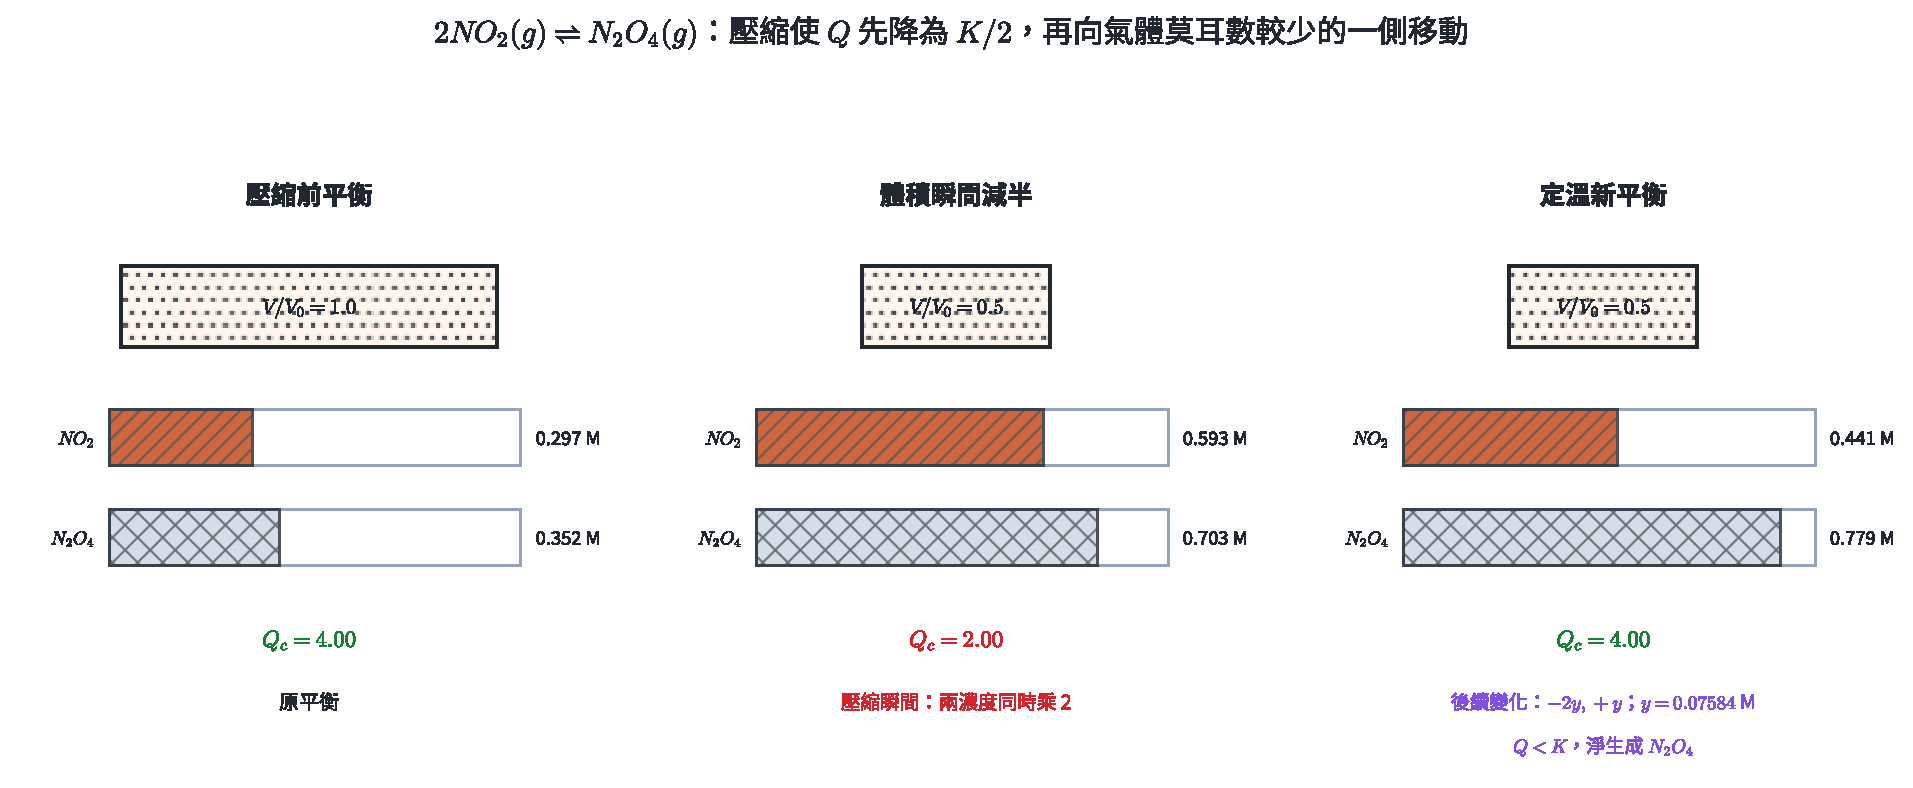
\includegraphics[width=0.99\linewidth,height=\textheight,keepaspectratio,alt={圖 8｜NO2/N2O4 平衡的體積減半計算：濃度先加倍，Q 由 4.00 降至 2.00，再由 −2y、+y 建立新平衡。}]{assets/選化III-1-壓縮NO2-N2O4平衡.pdf}
\caption{圖 8｜NO2/N2O4 平衡的體積減半計算：濃度先加倍，Q 由 4.00 降至 2.00，再由 −2y、+y 建立新平衡。}
\end{figure}

\begin{HandoutWorkedExample}

\subsection{示範 9｜精確計算壓縮後的新平衡}\label{ux793aux7bc4-9ux7cbeux78baux8a08ux7b97ux58d3ux7e2eux5f8cux7684ux65b0ux5e73ux8861}

沿用 \(2NO_2\rightleftharpoons N_2O_4\)、\(K_c=4.00\)。壓縮前 \([NO_2]=0.2965\)、\([N_2O_4]=0.3517\ \mathrm M\)。體積瞬間減半後為 \(0.5931\) 與 \(0.7035\ \mathrm M\)，

\[
Q_c=\frac{0.7035}{(0.5931)^2}=2.00<K_c.
\]

令後續生成 \(N_2O_4\) 的濃度為 \(y\)：

\[
4.00=\frac{0.7035+y}{(0.5931-2y)^2}.
\]

可行根 \(y=0.07584\ \mathrm M\)，新平衡 \([NO_2]=0.4414\ \mathrm M\)、\([N_2O_4]=0.7793\ \mathrm M\)。\([NO_2]+2[N_2O_4]\) 在後續反應前後皆為 \(2.000\ \mathrm M\)。

\end{HandoutWorkedExample}

惰性氣體效果取決於操作條件：定溫定容加入 He 時各反應氣體分壓不變，\(Q_p\) 不變；定溫定壓加入 He 時容器膨脹，各反應氣體分壓下降，系統依 \(\Delta n_g\) 判斷；反應兩側氣體係數總和相同時，等比例改變分壓後 \(Q_p\) 不變。

\subsection{3.3 溫度與平衡常數}\label{ux6eabux5ea6ux8207ux5e73ux8861ux5e38ux6578}

溫度改變指定反應的 \(K\)。把熱量寫入反應式可作方向判斷：放熱正反應升溫時偏向反應物，\(K\) 變小；吸熱正反應升溫時偏向產物，\(K\) 變大。

\begin{figure}
\centering
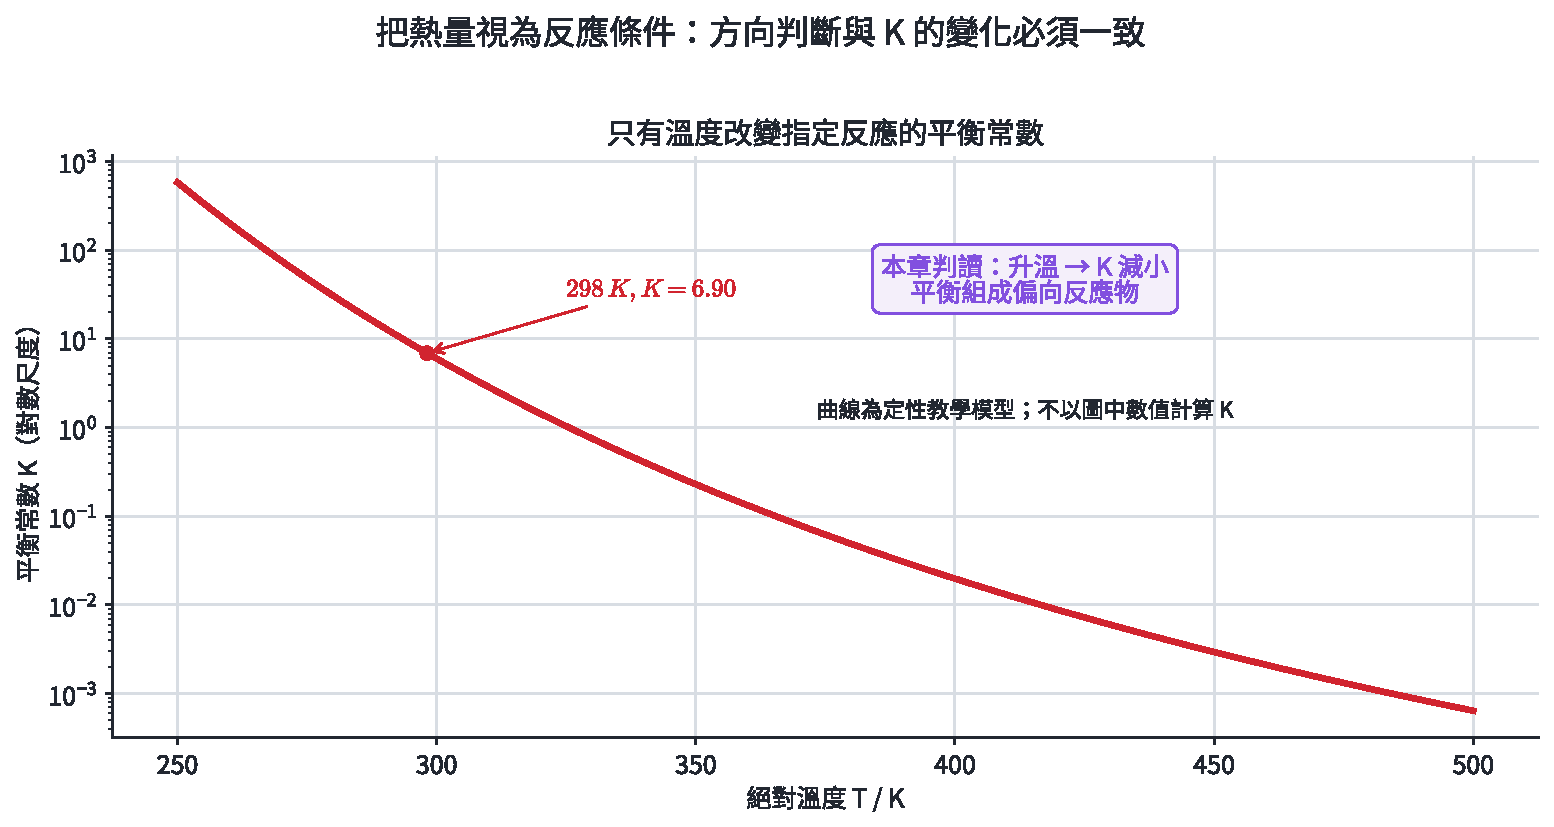
\includegraphics[width=0.94\linewidth,height=\textheight,keepaspectratio,alt={圖 9｜放熱反應的定性教學模型；溫度上升時 K 單調下降，本章只用曲線判讀方向。}]{assets/選化III-1-溫度改變平衡常數.pdf}
\caption{圖 9｜放熱反應的定性教學模型；溫度上升時 K 單調下降，本章只用曲線判讀方向。}
\end{figure}

\begin{HandoutWorkedExample}

\subsection{\texorpdfstring{示範 10｜由不同溫度的 \(K\) 判斷反應熱}{示範 10｜由不同溫度的 K 判斷反應熱}}\label{ux793aux7bc4-10ux7531ux4e0dux540cux6eabux5ea6ux7684-k-ux5224ux65b7ux53cdux61c9ux71b1}

某反應在 \(300\ \mathrm K\)、\(400\ \mathrm K\) 的 \(K\) 分別為 \(0.80\)、\(5.2\)。升溫使 \(K\) 增大，代表平衡組成中的產物相對增加，因此正反應吸熱。由 \(400\ \mathrm K\) 降回 \(300\ \mathrm K\)，淨反應偏向反應物，新的 \(K\) 回到 \(0.80\)。

\end{HandoutWorkedExample}

\subsection{3.4 催化劑與達平衡時間}\label{ux50acux5316ux5291ux8207ux9054ux5e73ux8861ux6642ux9593}

催化劑提供較低活化能路徑，正、逆反應都加速。反應物與產物的能量差不變，所以相同溫度下 \(K\) 與平衡組成不變；從同一初始組成出發，曲線較快進入相同平台。

\begin{figure}
\centering
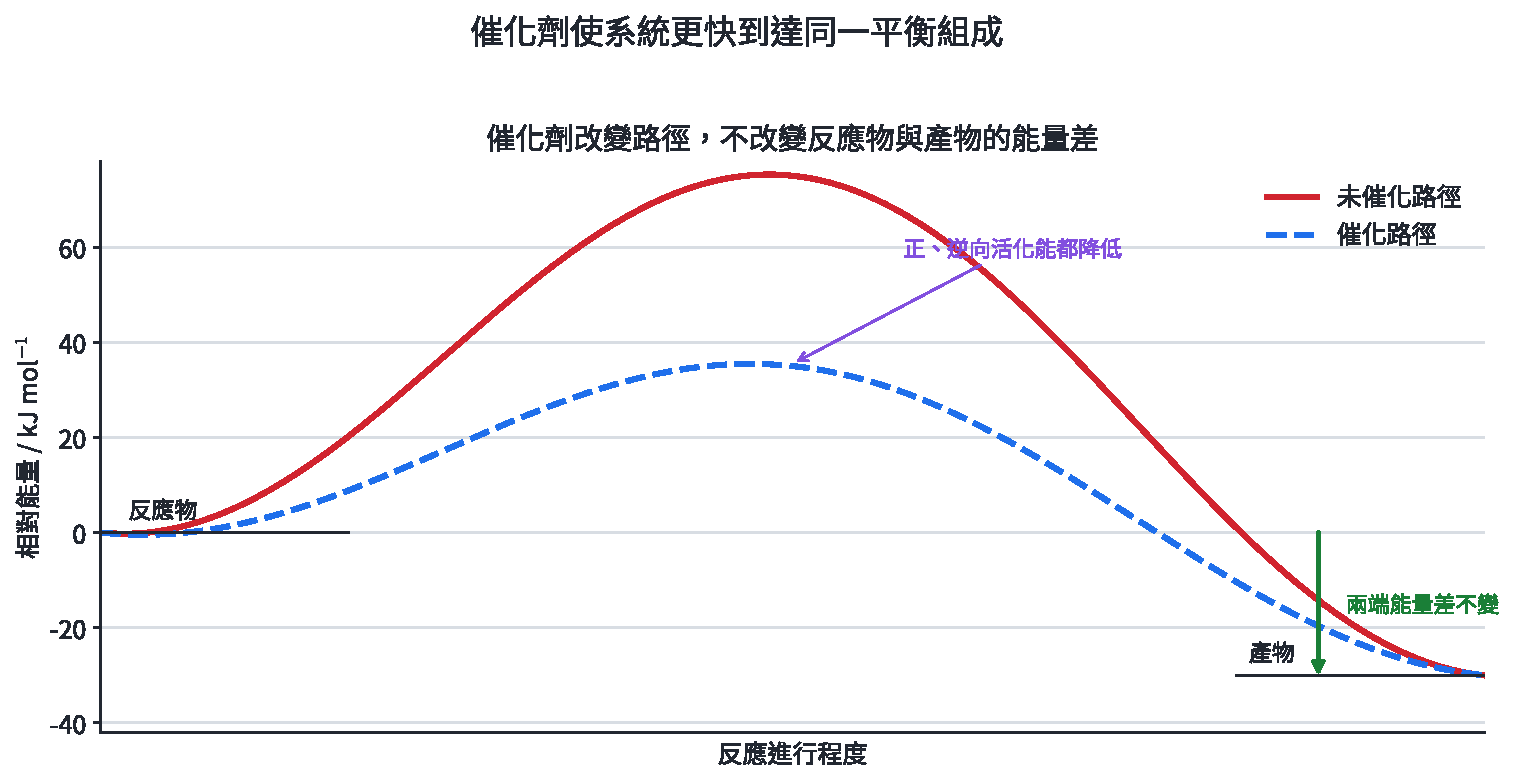
\includegraphics[width=0.94\linewidth,height=\textheight,keepaspectratio,alt={圖 10｜催化與未催化路徑的兩端能量相同，催化路徑峰值較低；因此 K 與平衡位置相同。}]{assets/選化III-1-催化劑與平衡.pdf}
\caption{圖 10｜催化與未催化路徑的兩端能量相同，催化路徑峰值較低；因此 K 與平衡位置相同。}
\end{figure}

\subsection{3.5 合成氨的多條件權衡}\label{ux5408ux6210ux6c28ux7684ux591aux689dux4ef6ux6b0aux8861}

\[
N_2(g)+3H_2(g)\rightleftharpoons2NH_3(g)+\text{熱}.
\]

低溫提高平衡產率，卻使反應變慢；高壓提高產率，也增加壓縮與耐壓設備成本。工業上採用適中溫度、高壓、鐵系催化劑，冷凝移除 \(NH_3\) 並循環未反應氣體。

\begin{figure}
\centering
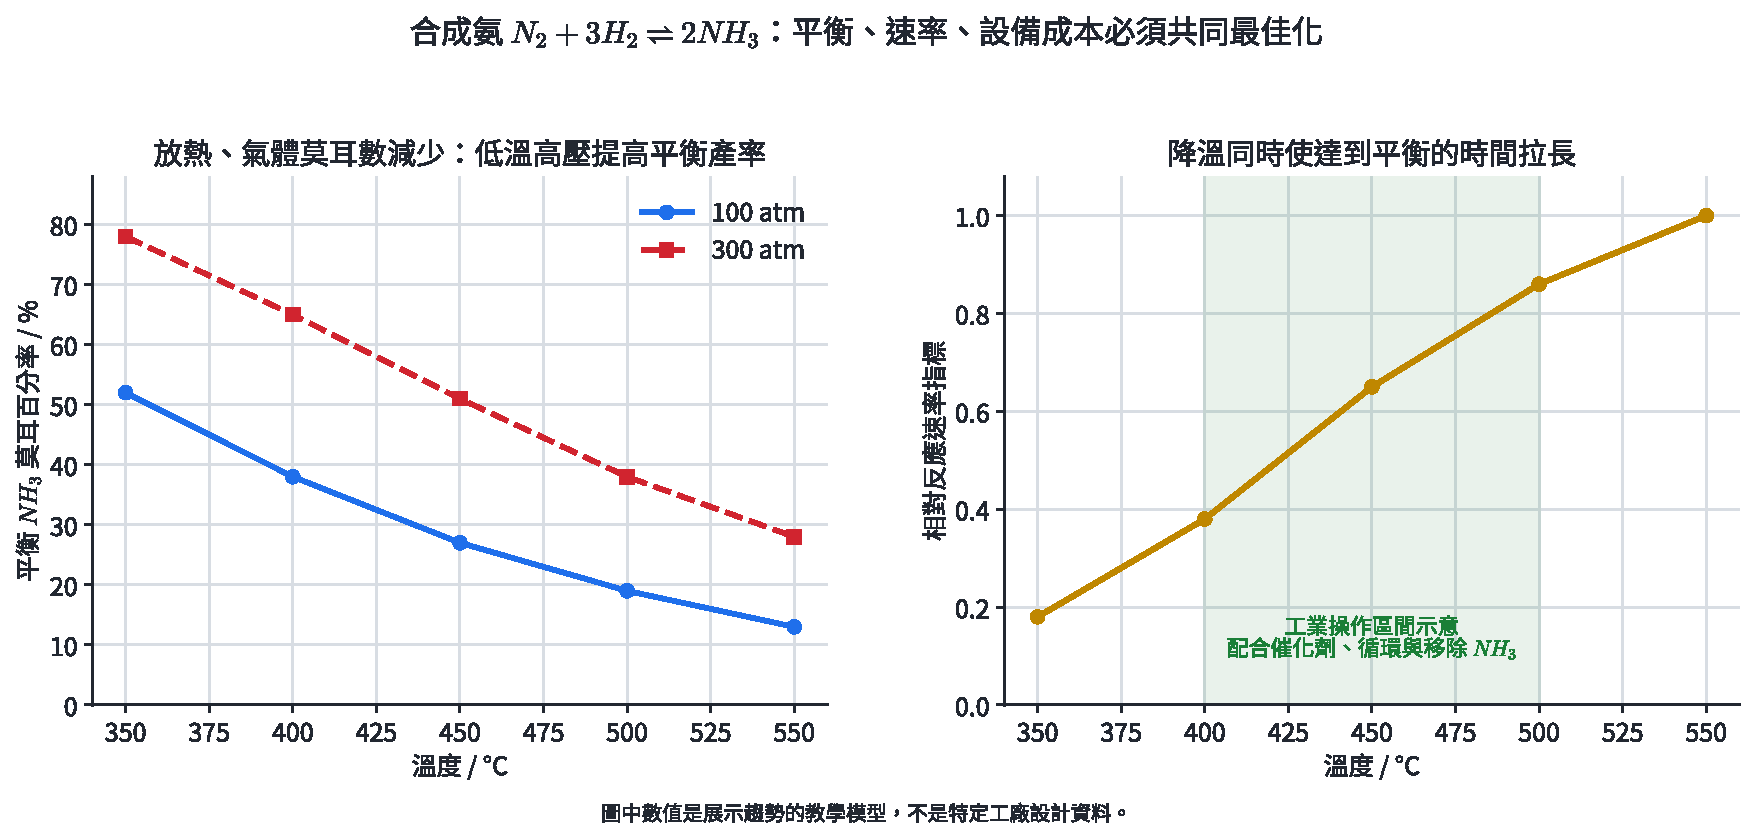
\includegraphics[width=0.98\linewidth,height=\textheight,keepaspectratio,alt={圖 11｜左圖是明示為教學模型的溫壓---平衡產率資料，右圖是相對速率；兩圖共同說明工業操作區間。}]{assets/選化III-1-合成氨條件權衡.pdf}
\caption{圖 11｜左圖是明示為教學模型的溫壓---平衡產率資料，右圖是相對速率；兩圖共同說明工業操作區間。}
\end{figure}

\begin{HandoutWorkedExample}

\subsection{\texorpdfstring{示範 11｜辨認條件對 \(Q\)、\(K\) 與時間的不同作用}{示範 11｜辨認條件對 Q、K 與時間的不同作用}}\label{ux793aux7bc4-11ux8fa8ux8a8dux689dux4ef6ux5c0d-qk-ux8207ux6642ux9593ux7684ux4e0dux540cux4f5cux7528}

合成氨系統已達平衡：

\begin{enumerate}
\def\labelenumi{\arabic{enumi}.}
\tightlist
\item
  定溫定容加入 \(H_2\)：\(Q_p\) 分母增大而 \(Q_p<K_p\)，向右；\(K_p\) 不變。
\item
  升溫：放熱正反應的 \(K_p\) 變小，平衡向左；正、逆速率常都先變快。
\item
  加催化劑：正、逆反應都更快，平衡組成不變，達平衡時間縮短。
\end{enumerate}

\end{HandoutWorkedExample}

\subsection{練習 3}\label{ux7df4ux7fd2-3}

\begin{enumerate}
\def\labelenumi{\arabic{enumi}.}
\tightlist
\item
  \(N_2+3H_2\rightleftharpoons2NH_3\) 定溫平衡後加入 \(NH_3\)，寫出 \(Q_p\) 的瞬間變化、方向與 \(K_p\) 是否改變。
\item
  \(CO+H_2O\rightleftharpoons CO_2+H_2\) 定溫壓縮至體積一半。以 \(Q_p\) 說明是否移動。
\item
  對 \(N_2O_4\rightleftharpoons2NO_2\)，比較定溫定容加入 He 與定溫定壓加入 He。
\item
  某反應的 \(K\)：300 K 時 12.0、400 K 時 3.4、500 K 時 1.2。判斷正反應吸放熱與升溫時方向。
\item
  畫出有、無催化劑時產物濃度對時間的兩條曲線，標示平台值與時間關係。
\item
  對 \(2NO_2\rightleftharpoons N_2O_4+\text{熱}\)，敘述壓縮與加熱時紅棕色的立即變化及後續變化。
\end{enumerate}

\subsection{練習 3 解析}\label{ux7df4ux7fd2-3-ux89e3ux6790}

\begin{enumerate}
\def\labelenumi{\arabic{enumi}.}
\tightlist
\item
  \(Q_p=P_{NH_3}^2/(P_{N_2}P_{H_2}^3)\)。加入 \(NH_3\) 使 \(Q_p>K_p\)，淨反應向左；溫度不變，所以 \(K_p\) 不變。
\item
  各分壓都加倍，\(Q_p'=(2P_{CO_2})(2P_{H_2})/[(2P_{CO})(2P_{H_2O})]=Q_p=K_p\)，所以無移動。
\item
  定容加入 He 時各反應氣體分壓不變。定壓加入 He 時體積增大、分壓下降，\(Q_p=P_{NO_2}^2/P_{N_2O_4}\) 下降，向右移動。
\item
  升溫使 \(K\) 下降，正反應放熱；升溫後平衡向反應物側移動。
\item
  兩曲線到達同一平台；有催化劑者初期斜率較大、較早進入平台。
\item
  壓縮：\(NO_2\) 濃度立即升高而變深，接著向右形成 \(N_2O_4\) 而逐漸變淡。定容加熱：平衡向吸熱的左側移動，\(NO_2\) 增加而逐漸變深。
\end{enumerate}

\clearpage

\section{4. 溶解平衡與溶度積}\label{ux6eb6ux89e3ux5e73ux8861ux8207ux6eb6ux5ea6ux7a4d}

\subsection{4.1 難溶鹽的動態溶解平衡}\label{ux96e3ux6eb6ux9e7dux7684ux52d5ux614bux6eb6ux89e3ux5e73ux8861}

難溶鹽放入水中，晶格表面的離子持續進入溶液，溶液中的離子也持續回到晶格。當溶解速率等於結晶速率時，固體與飽和溶液達到動態平衡。例如

\[
AgCl(s)\rightleftharpoons Ag^+(aq)+Cl^-(aq).
\]

純固體活性為 1，\textbf{溶度積常數}為

\[
K_{sp}=[Ag^+][Cl^-].
\]

對一般鹽 \(A_xB_y(s)\rightleftharpoons xA^{m+}+yB^{n-}\)，

\[
K_{sp}=[A^{m+}]^x[B^{n-}]^y.
\]

\(K_{sp}\) 只在指定溫度下描述飽和溶液。溶液中沒有固體且離子積小於 \(K_{sp}\) 時屬未飽和；此時把現有濃度相乘得到的是 \(Q_{sp}\)。

\subsection{4.2 莫耳溶解度與化學計量}\label{ux83abux8033ux6eb6ux89e3ux5ea6ux8207ux5316ux5b78ux8a08ux91cf}

\textbf{莫耳溶解度} \(s\) 是每公升飽和溶液中溶解鹽的莫耳數。離子濃度需乘上解離係數：

\[
AB(s)\rightleftharpoons A^++B^-:\quad [A^+]=s, [B^-]=s, K_{sp}=s^2,
\]

\[
AB_2(s)\rightleftharpoons A^{2+}+2B^-:\quad [A^{2+}]=s, [B^-]=2s, K_{sp}=4s^3.
\]

\begin{figure}
\centering
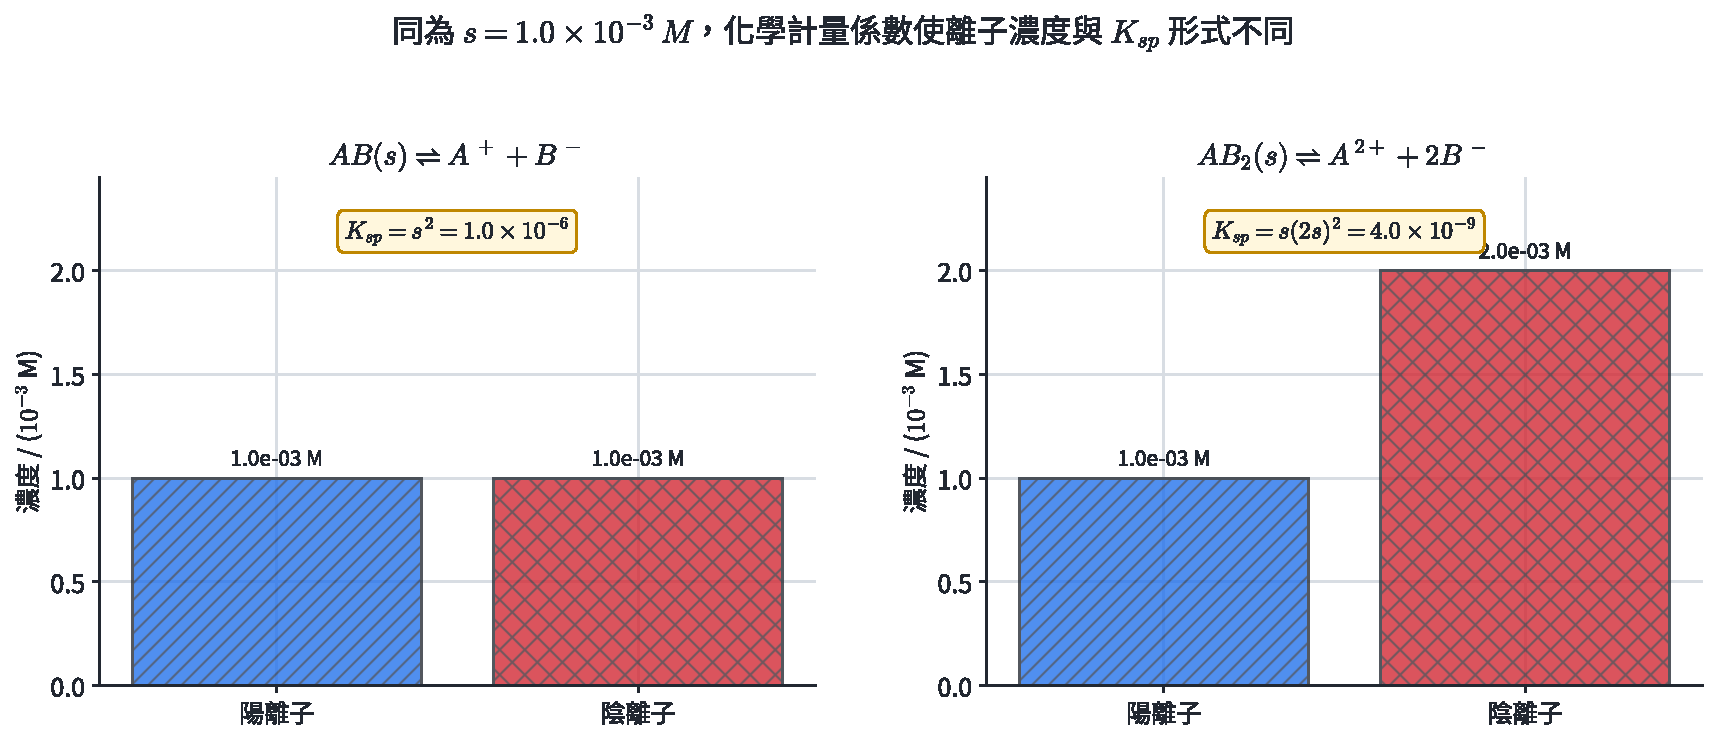
\includegraphics[width=0.96\linewidth,height=\textheight,keepaspectratio,alt={圖 12｜\textbackslash mathrm\{AB\} 與 \textbackslash mathrm\{AB\_2\} 都取 s=10\^{}\{-3\}\textbackslash{} \textbackslash mathrm M；陰離子濃度與 K\_\{sp\} 的次方因化學計量不同。}]{assets/選化III-1-溶度積與莫耳溶解度.pdf}
\caption{圖 12｜\(\mathrm{AB}\) 與 \(\mathrm{AB_2}\) 都取 \(s=10^{-3}\ \mathrm M\)；陰離子濃度與 \(K_{sp}\) 的次方因化學計量不同。}
\end{figure}

\begin{HandoutWorkedExample}

\subsection{\texorpdfstring{示範 12｜由 \(K_{sp}\) 求 \(PbI_2\) 的莫耳溶解度}{示範 12｜由 K\_\{sp\} 求 PbI\_2 的莫耳溶解度}}\label{ux793aux7bc4-12ux7531-k_sp-ux6c42-pbi_2-ux7684ux83abux8033ux6eb6ux89e3ux5ea6}

在某溫度下 \(K_{sp}(PbI_2)=7.1\times10^{-9}\)：

\[
PbI_2(s)\rightleftharpoons Pb^{2+}+2I^-.
\]

若在純水中的莫耳溶解度為 \(s\)，則

\[
K_{sp}=s(2s)^2=4s^3.
\]

\[
s=\left(\frac{7.1\times10^{-9}}4\right)^{1/3}
=1.21\times10^{-3}\ \mathrm M.
\]

因此 \([Pb^{2+}]=1.21\times10^{-3}\ \mathrm M\)，\([I^-]=2.42\times10^{-3}\ \mathrm M\)；回代濃度與係數相符。

\end{HandoutWorkedExample}

\subsection{4.3 同離子效應}\label{ux540cux96e2ux5b50ux6548ux61c9}

若溶液原本已有與難溶鹽相同的離子，溶解反應的 \(Q_{sp}\) 增大，平衡向固體側移動，莫耳溶解度下降，稱為\textbf{同離子效應}。

對 AgCl 加入初始濃度 \(c_0\) 的 \(Cl^-\)，若另溶解 \(s\)：

\[
K_{sp}=s(c_0+s).
\]

\begin{figure}
\centering
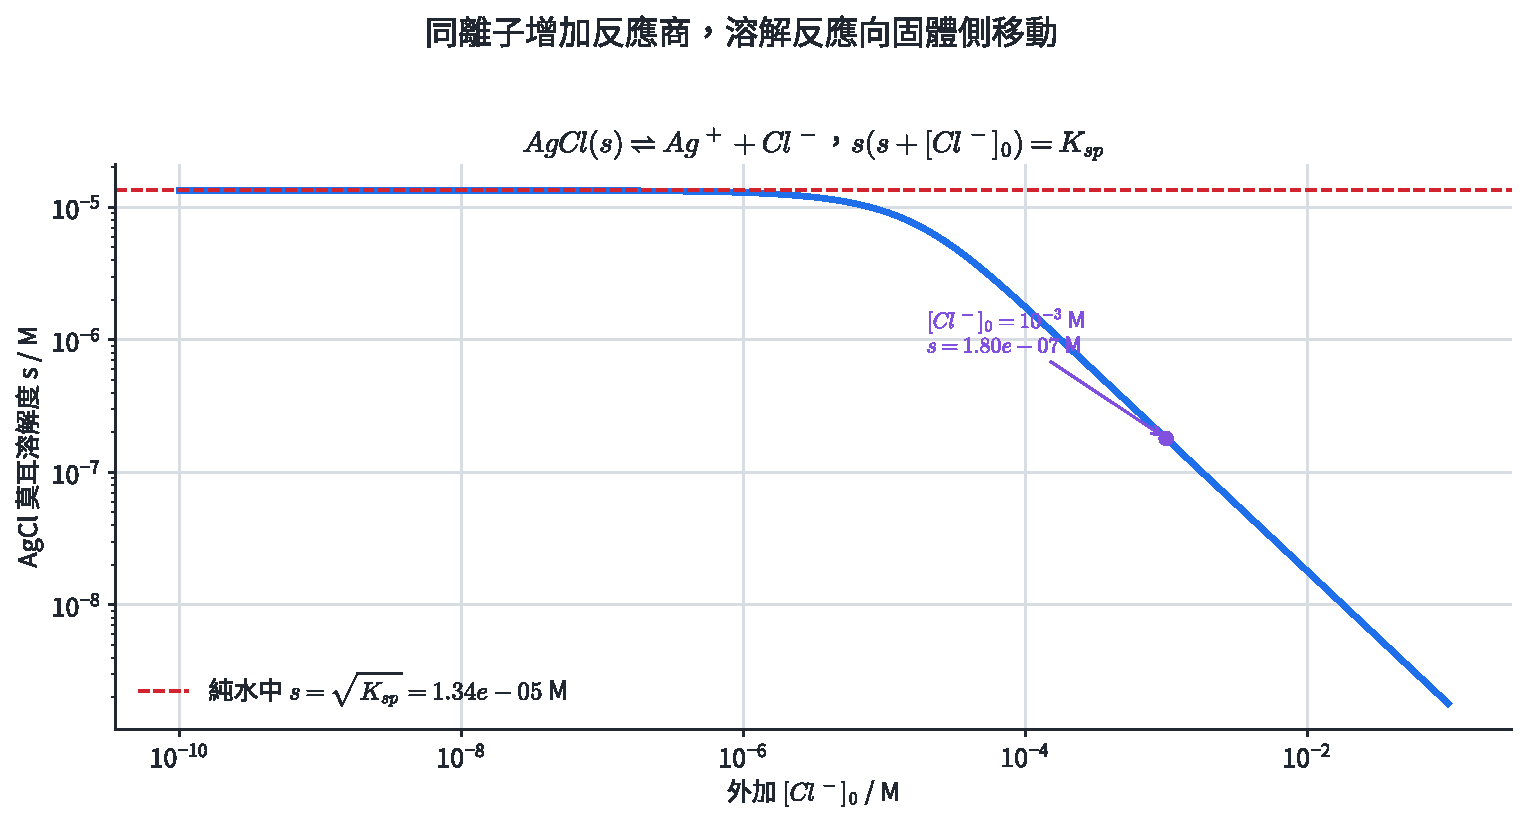
\includegraphics[width=0.94\linewidth,height=\textheight,keepaspectratio,alt={圖 13｜\textbackslash mathrm\{AgCl\} 的精確解 s(s+c\_0)=K\_\{sp\}；外加 \textbackslash mathrm\{Cl\^{}-\} 越多，莫耳溶解度單調下降。}]{assets/選化III-1-同離子與AgCl溶解度.pdf}
\caption{圖 13｜\(\mathrm{AgCl}\) 的精確解 \(s(s+c_0)=K_{sp}\)；外加 \(\mathrm{Cl^-}\) 越多，莫耳溶解度單調下降。}
\end{figure}

\begin{HandoutWorkedExample}

\subsection{\texorpdfstring{示範 13｜AgCl 在含 \(Cl^-\) 溶液中的溶解度}{示範 13｜AgCl 在含 Cl\^{}- 溶液中的溶解度}}\label{ux793aux7bc4-13agcl-ux5728ux542b-cl--ux6eb6ux6db2ux4e2dux7684ux6eb6ux89e3ux5ea6}

\(K_{sp}(AgCl)=1.8\times10^{-10}\)。求 AgCl 在 \(1.00\times10^{-3}\ \mathrm M\) NaCl 中的 \(s\)。

\[
s(1.00\times10^{-3}+s)=1.8\times10^{-10}.
\]

解二次式得

\[
s=1.80\times10^{-7}\ \mathrm M.
\]

因 \(s/(1.00\times10^{-3})=1.80\times10^{-4}\)，可用 \(1.00\times10^{-3}+s\approx1.00\times10^{-3}\) 近似；近似值同為 \(1.8\times10^{-7}\ \mathrm M\)。近似是否成立要以所得 \(s\) 回頭比較，不能只看題目數字大小。

\end{HandoutWorkedExample}

\begin{HandoutWorkedExample}

\subsection{\texorpdfstring{示範 14｜比較 \(K_{sp}\) 與溶解度時先看化學計量}{示範 14｜比較 K\_\{sp\} 與溶解度時先看化學計量}}\label{ux793aux7bc4-14ux6bd4ux8f03-k_sp-ux8207ux6eb6ux89e3ux5ea6ux6642ux5148ux770bux5316ux5b78ux8a08ux91cf}

某溫度下 \(K_{sp}(AB)=4.0\times10^{-8}\)，\(K_{sp}(AB_2)=3.2\times10^{-11}\)。

對 AB：

\[
s=\sqrt{4.0\times10^{-8}}=2.0\times10^{-4}\ \mathrm M.
\]

對 \(AB_2\)：

\[
4s^3=3.2\times10^{-11}
\Rightarrow s=2.0\times10^{-4}\ \mathrm M.
\]

兩者 \(K_{sp}\) 相差三個數量級，莫耳溶解度卻相同。直接比較 \(K_{sp}\) 大小只適用於解離化學計量形式相同的鹽。

\end{HandoutWorkedExample}

\subsection{4.4 直接用途與模型限制}\label{ux76f4ux63a5ux7528ux9014ux8207ux6a21ux578bux9650ux5236-1}

調整共同離子可控制藥物結晶、礦物析出、鍋爐水垢與金屬鹽回收。只用 \(K_{sp}\) 的簡化模型假設離子以自由水合離子存在且溶液近理想；高離子強度、錯離子形成、酸鹼反應與多晶型會改變實際溶解度。題目若提供配位或酸鹼資訊，需把相關平衡一併列入。

\subsection{練習 4}\label{ux7df4ux7fd2-4}

\begin{enumerate}
\def\labelenumi{\arabic{enumi}.}
\tightlist
\item
  \(K_{sp}(AgBr)=5.0\times10^{-13}\)，求其在純水中的莫耳溶解度。
\item
  \(K_{sp}[Mg(OH)_2]=1.8\times10^{-11}\)，求純水中的莫耳溶解度與 \([OH^-]\)。
\item
  \(K_{sp}(AgCl)=1.8\times10^{-10}\)。估算在 \(0.010\ \mathrm M\) NaCl 中的莫耳溶解度，並檢查近似。
\item
  飽和 AgCl 溶液中仍有固體。加入等體積純水後，立即的 \(Q_{sp}\) 與 \(K_{sp}\) 關係如何？之後固體量與離子濃度如何變化？
\item
  某鹽的 \(K_{sp}\) 在 20°C 為 \(2.0\times10^{-9}\)，在 50°C 為 \(8.0\times10^{-9}\)。判斷其溶解反應吸放熱，並說明升溫對溶解度的影響。
\end{enumerate}

\subsection{練習 4 解析}\label{ux7df4ux7fd2-4-ux89e3ux6790}

\begin{enumerate}
\def\labelenumi{\arabic{enumi}.}
\item
  AgBr 是 1:1 鹽，\(K_{sp}=s^2\)：

  \[
  s=\sqrt{5.0\times10^{-13}}=7.1\times10^{-7}\ \mathrm M.
  \]
\item
  \(Mg(OH)_2\rightleftharpoons Mg^{2+}+2OH^-\)，所以 \(K_{sp}=s(2s)^2=4s^3\)：

  \[
  s=\left(\frac{1.8\times10^{-11}}4\right)^{1/3}=1.65\times10^{-4}\ \mathrm M,
  \]

  \([OH^-]=2s=3.30\times10^{-4}\ \mathrm M\)。
\item
  \(s(0.010+s)=1.8\times10^{-10}\)。取 \(s\ll0.010\)：

  \[
  s\approx\frac{1.8\times10^{-10}}{0.010}=1.8\times10^{-8}\ \mathrm M.
  \]

  \(s/0.010=1.8\times10^{-6}\)，近似成立。
\item
  稀釋使兩離子濃度都減半，\(Q_{sp}\) 立即變成原來的 \(1/4\)，所以 \(Q_{sp}<K_{sp}\)。之後部分固體溶解，使離子濃度上升直到乘積回到 \(K_{sp}\)；固體量減少。只要固體仍存在，最後在同溫下仍是飽和濃度。
\item
  升溫使 \(K_{sp}\) 增大，代表溶解平衡偏向溶液離子，溶解反應吸熱；升溫通常提高莫耳溶解度。
\end{enumerate}

\section{5. 離子沉澱、分離與確認}\label{ux96e2ux5b50ux6c89ux6fb1ux5206ux96e2ux8207ux78baux8a8d}

\subsection{5.1 離子積與沉澱條件}\label{ux96e2ux5b50ux7a4dux8207ux6c89ux6fb1ux689dux4ef6}

把混合後的當下離子濃度代入溶度積形式，得到\textbf{離子積} \(Q_{sp}\)：

\[
\begin{aligned}
Q_{sp}<K_{sp}&:\ \text{未飽和，無沉澱生成},\\
Q_{sp}=K_{sp}&:\ \text{飽和或剛達沉澱門檻},\\
Q_{sp}>K_{sp}&:\ \text{過飽和，生成沉澱直到回到平衡}.
\end{aligned}
\]

混合溶液時先用總體積求混合後濃度，再算 \(Q_{sp}\)。出現沉澱後，剩餘離子濃度由化學計量、物料守恆與 \(K_{sp}\) 共同決定。

\begin{HandoutWorkedExample}

\subsection{示範 15｜混合後是否生成 AgCl}\label{ux793aux7bc4-15ux6df7ux5408ux5f8cux662fux5426ux751fux6210-agcl}

等體積混合 \(2.00\times10^{-4}\ \mathrm M\) AgNO\(_3\) 與 \(1.00\times10^{-3}\ \mathrm M\) NaCl。混合後

\[
[Ag^+]=1.00\times10^{-4}\ \mathrm M,\qquad
[Cl^-]=5.00\times10^{-4}\ \mathrm M.
\]

\[
Q_{sp}=(1.00\times10^{-4})(5.00\times10^{-4})=5.00\times10^{-8}.
\]

\(Q_{sp}>K_{sp}(AgCl)=1.8\times10^{-10}\)，所以生成 AgCl 沉澱。這個判斷只回答「會不會開始沉澱」；平衡後剩餘濃度需另做物料守恆。

\end{HandoutWorkedExample}

\subsection{5.2 起始沉澱濃度與選擇分離}\label{ux8d77ux59cbux6c89ux6fb1ux6fc3ux5ea6ux8207ux9078ux64c7ux5206ux96e2}

逐漸加入沉澱劑時，每種鹽開始沉澱都有臨界濃度。若離子 X 與沉澱劑 M 形成 \(MX\)：

\[
[M]_{\mathrm{start}}=\frac{K_{sp}}{[X]}.
\]

若形成 \(M_2Y\)：

\[
[M]_{\mathrm{start}}=\sqrt{\frac{K_{sp}}{[Y]}}.
\]

先達門檻的鹽先沉澱；兩門檻之間是選擇分離的操作窗。

\begin{figure}
\centering
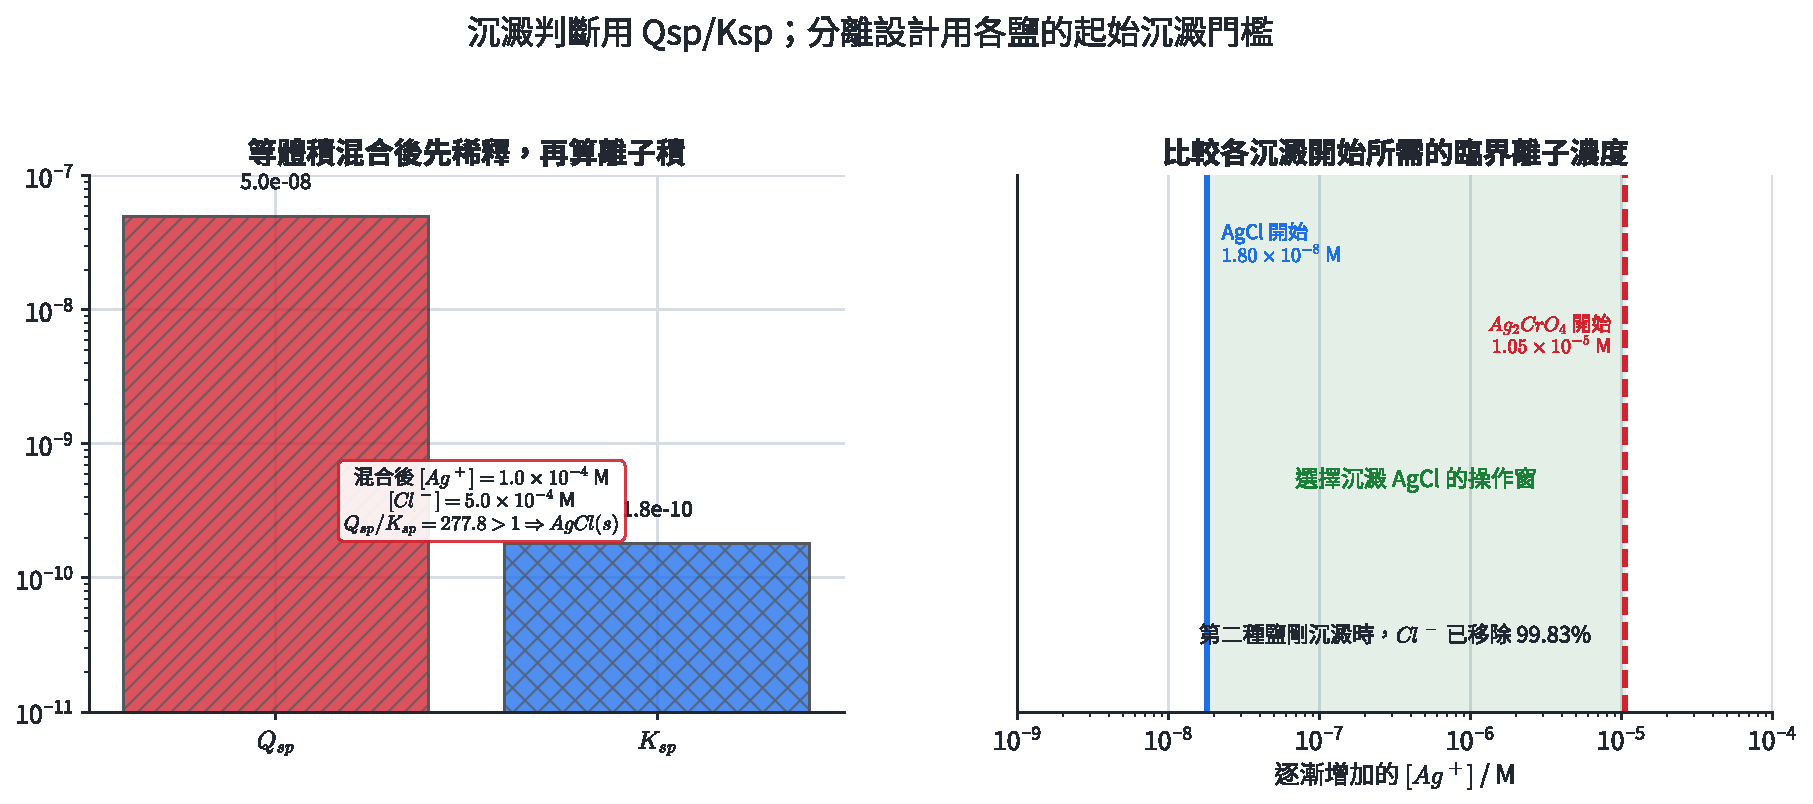
\includegraphics[width=0.99\linewidth,height=\textheight,keepaspectratio,alt={圖 14｜左圖比較混合後 Q\_\{sp\} 與 K\_\{sp\}；右圖以 \textbackslash mathrm\{Ag\^{}+\} 臨界濃度畫出 \textbackslash mathrm\{AgCl\} 與 \textbackslash mathrm\{Ag\_2CrO\_4\} 的選擇沉澱窗。}]{assets/選化III-1-離子積與選擇沉澱.pdf}
\caption{圖 14｜左圖比較混合後 \(Q_{sp}\) 與 \(K_{sp}\)；右圖以 \(\mathrm{Ag^+}\) 臨界濃度畫出 \(\mathrm{AgCl}\) 與 \(\mathrm{Ag_2CrO_4}\) 的選擇沉澱窗。}
\end{figure}

\begin{HandoutWorkedExample}

\subsection{\texorpdfstring{示範 16｜設計 \(Cl^-\)、\(CrO_4^{2-}\) 的選擇沉澱}{示範 16｜設計 Cl\^{}-、CrO\_4\^{}\{2-\} 的選擇沉澱}}\label{ux793aux7bc4-16ux8a2dux8a08-cl-cro_42--ux7684ux9078ux64c7ux6c89ux6fb1}

溶液初始 \([Cl^-]=[CrO_4^{2-}]=0.010\ \mathrm M\)，逐漸加入 Ag\(^+\)。取

\[
K_{sp}(AgCl)=1.8\times10^{-10},\qquad
K_{sp}(Ag_2CrO_4)=1.1\times10^{-12}.
\]

AgCl 開始沉澱時

\[
[Ag^+]=\frac{1.8\times10^{-10}}{0.010}=1.8\times10^{-8}\ \mathrm M.
\]

\(Ag_2CrO_4\) 開始沉澱時

\[
[Ag^+]=\sqrt{\frac{1.1\times10^{-12}}{0.010}}
=1.05\times10^{-5}\ \mathrm M.
\]

因此 AgCl 先沉澱。在第二種鹽剛開始沉澱時，

\[
[Cl^-]=\frac{1.8\times10^{-10}}{1.05\times10^{-5}}
=1.72\times10^{-5}\ \mathrm M,
\]

已移除的 \(Cl^-\) 比例為 \(1-(1.72\times10^{-5}/0.010)=99.83\%\)。這項結果假設體積變化可忽略、沒有錯離子或共沉澱。

\end{HandoutWorkedExample}

\subsection{5.3 沉澱確認與證據強度}\label{ux6c89ux6fb1ux78baux8a8dux8207ux8b49ux64daux5f37ux5ea6}

沉澱的顏色、酸鹼溶解性與配位溶解性可提供離子確認線索。可靠流程要同時包含空白試驗、已知陽性對照、選擇性試劑與後續確認反應。單一白色沉澱通常對應多種可能離子，因此推論應寫成「結果支持某離子存在」，再用第二個獨立證據縮小範圍。

沉澱分離直接應用於飲用水軟化、硫酸根分析、重金屬廢水處理與礦物精製。硝酸銀具氧化性並可灼傷皮膚、鉻酸鹽含六價鉻且具高危害；示範資料只用於計算，實作需依學校核准的微量方案、通風與個人防護，含銀、鉛、鉻及其他重金屬沉澱與濾液分流收集，不排入水槽。

\begin{HandoutWorkedExample}

\subsection{示範 17｜把沉澱觀察寫成證據鏈}\label{ux793aux7bc4-17ux628aux6c89ux6fb1ux89c0ux5bdfux5bebux6210ux8b49ux64daux93c8}

未知液加入含 \(Ba^{2+}\) 試劑後出現白色沉澱；另一份未知液先酸化再加同試劑，仍出現白色沉澱。可作如下推理：

\begin{enumerate}
\def\labelenumi{\arabic{enumi}.}
\tightlist
\item
  觀察：兩份試樣均形成白色固體。
\item
  證據：酸化可消耗 \(CO_3^{2-}\) 並釋出 \(CO_2\)，卻不會同樣移除 \(SO_4^{2-}\)。
\item
  推論：酸化後仍沉澱的結果支持 \(SO_4^{2-}\) 存在，並降低「只有 \(CO_3^{2-}\)」的可能性。
\item
  控制：以純水作空白、已知硫酸鹽作陽性對照，保持酸量與試劑量一致。
\end{enumerate}

若題目提供其他可與 \(Ba^{2+}\) 形成難溶鹽的陰離子，仍需加入相應排除步驟。

\end{HandoutWorkedExample}

\subsection{練習 5}\label{ux7df4ux7fd2-5}

\begin{enumerate}
\def\labelenumi{\arabic{enumi}.}
\tightlist
\item
  混合 \(25.0\ \mathrm{mL}\)、\(4.0\times10^{-4}\ \mathrm M\) AgNO\(_3\) 與 \(75.0\ \mathrm{mL}\)、\(2.0\times10^{-4}\ \mathrm M\) NaCl。以 \(K_{sp}=1.8\times10^{-10}\) 判斷是否沉澱。
\item
  溶液中 \([Br^-]=2.0\times10^{-3}\ \mathrm M\)，\(K_{sp}(AgBr)=5.0\times10^{-13}\)。求 AgBr 開始沉澱所需 \([Ag^+]\)。
\item
  某溶液含等濃度 \(SO_4^{2-}\)、\(CO_3^{2-}\)，逐漸加入 \(Ba^{2+}\)。若 \(K_{sp}(BaSO_4)=1.1\times10^{-10}\)、\(K_{sp}(BaCO_3)=5.0\times10^{-9}\)，何者先沉澱？
\item
  在 \(Ag_2CrO_4\) 剛開始沉澱、\([Ag^+]=1.0\times10^{-5}\ \mathrm M\) 時，利用 \(K_{sp}(AgCl)=1.8\times10^{-10}\) 求殘餘 \([Cl^-]\)。若初始 \([Cl^-]=0.020\ \mathrm M\)，求移除百分率。
\item
  寫出以沉澱反應確認 \(SO_4^{2-}\) 的一組「空白、陽性對照、未知樣」安排，並寫出一項安全／廢液處置。
\end{enumerate}

\subsection{練習 5 解析}\label{ux7df4ux7fd2-5-ux89e3ux6790}

\begin{enumerate}
\def\labelenumi{\arabic{enumi}.}
\item
  總體積 \(0.100\ \mathrm L\)：

  \[
  [Ag^+]=\frac{(0.0250)(4.0\times10^{-4})}{0.100}=1.0\times10^{-4}\ \mathrm M,
  \]

  \[
  [Cl^-]=\frac{(0.0750)(2.0\times10^{-4})}{0.100}=1.5\times10^{-4}\ \mathrm M.
  \]

  \(Q_{sp}=1.5\times10^{-8}>K_{sp}\)，生成 AgCl。
\item
  \([Ag^+]_{\mathrm{start}}=K_{sp}/[Br^-]=(5.0\times10^{-13})/(2.0\times10^{-3})=2.5\times10^{-10}\ \mathrm M\)。
\item
  兩鹽都是 1:1，陰離子初濃度相同，所需 \([Ba^{2+}]\) 與 \(K_{sp}\) 成正比。\(BaSO_4\) 的門檻較低，先沉澱。
\item
  \([Cl^-]=K_{sp}/[Ag^+]=1.8\times10^{-5}\ \mathrm M\)。移除率

  \[
  \left(1-\frac{1.8\times10^{-5}}{0.020}\right)\times100\%=99.91\%.
  \]
\item
  空白以純水加同量酸與 \(Ba^{2+}\) 試劑；陽性對照以已知硫酸鹽作相同處理；未知樣先酸化再加試劑，比較是否形成白色沉澱。使用護目鏡與手套，含鋇／重金屬的沉澱和濾液收集至指定無機廢液桶。
\end{enumerate}

\section{6. 章末分層題}\label{ux7ae0ux672bux5206ux5c64ux984c}

\subsection{基礎題 1--6}\label{ux57faux790eux984c-16}

\begin{enumerate}
\def\labelenumi{\arabic{enumi}.}
\tightlist
\item
  用「速率」與「濃度」各寫一句動態平衡的定義。
\item
  寫出 \(2SO_2(g)+O_2(g)\rightleftharpoons2SO_3(g)\) 的 \(K_c\)。
\item
  已知 \(A\rightleftharpoons B\) 的 \(K=25\)，求 \(2B\rightleftharpoons2A\) 的平衡常數。
\item
  \(A\rightleftharpoons B\) 的 \(K_c=3.0\)。某時刻 \([A]=0.40\ \mathrm M\)、\([B]=0.60\ \mathrm M\)，判斷淨反應方向。
\item
  \(A\rightleftharpoons B\) 的 \(K_c=3.0\)，初始 \([A]=1.00\ \mathrm M\)、\([B]=0\)。求平衡濃度。
\item
  \(N_2+3H_2\rightleftharpoons2NH_3\) 在 \(700\ \mathrm K\) 的 \(K_c=5.0\times10^3\)。求 \(K_p\)，取 \(R=0.082057\)。
\end{enumerate}

\subsection{核心題 7--12}\label{ux6838ux5fc3ux984c-712}

\begin{enumerate}
\def\labelenumi{\arabic{enumi}.}
\setcounter{enumi}{6}
\tightlist
\item
  合成氨平衡在定溫定容下加入 \(N_2\)。寫出 \(Q_p\) 的變化、方向、新平衡 \(N_2\) 分壓相對於原平衡的大小，以及 \(K_p\) 是否改變。
\item
  對 \(N_2O_4\rightleftharpoons2NO_2\)，說明定溫定容加入 He 與定溫定壓加入 He 的差異。
\item
  某放熱可逆反應加入催化劑後再升溫。分別說明達平衡時間、\(K\) 與產物平衡比例的變化。
\item
  \(K_{sp}(MgF_2)=6.4\times10^{-9}\)。求其在純水中的莫耳溶解度。
\item
  \(K_{sp}(AgCl)=1.8\times10^{-10}\)。估算 AgCl 在 \(0.010\ \mathrm M\) NaCl 中的莫耳溶解度。
\item
  混合 \(20.0\ \mathrm{mL}\)、\(1.0\times10^{-3}\ \mathrm M\) AgNO\(_3\) 與 \(80.0\ \mathrm{mL}\)、\(5.0\times10^{-4}\ \mathrm M\) NaCl。判斷是否生成 AgCl。
\end{enumerate}

\subsection{跨節整合題 13--16}\label{ux8de8ux7bc0ux6574ux5408ux984c-1316}

\begin{enumerate}
\def\labelenumi{\arabic{enumi}.}
\setcounter{enumi}{12}
\tightlist
\item
  密閉注射筒中 \(2NO_2(g)\rightleftharpoons N_2O_4(g)+\text{熱}\) 已平衡。先在定溫下把體積壓成一半，待新平衡後再於定容下升溫。依序寫出每一步的 \(Q/K\)、顏色變化、\(K\) 是否改變，並列兩項必要安全措施。
\item
  比色法研究 \(Fe^{3+}+SCN^-\rightleftharpoons FeSCN^{2+}\)。標準液 \([FeSCN^{2+}]=1.20\times10^{-4}\ \mathrm M\)、光徑 \(1.00\ \mathrm{cm}\)；未知平衡液光徑 \(2.40\ \mathrm{cm}\) 時吸光度相同。未知液初始 \([Fe^{3+}]=1.00\times10^{-3}\ \mathrm M\)、\([SCN^-]=1.50\times10^{-4}\ \mathrm M\)。求平衡濃度與 \(K_c\)，並寫一個控制變因、一個模型限制與廢液去向。
\item
  合成氨的教學資料如下。判斷 450°C 下壓力效果、300 atm 下溫度效果，並提出同時考慮平衡、速率與分離的操作策略。
\end{enumerate}

{\def\LTcaptype{none} % do not increment counter
\begin{longtable}[]{@{}lrrr@{}}
\toprule\noalign{}
條件 & 400°C & 450°C & 500°C \\
\midrule\noalign{}
\endhead
\bottomrule\noalign{}
\endlastfoot
100 atm 的平衡 NH\(_3\) 比例 & 38\% & 27\% & 19\% \\
300 atm 的平衡 NH\(_3\) 比例 & 65\% & 51\% & 38\% \\
\end{longtable}
}

\begin{enumerate}
\def\labelenumi{\arabic{enumi}.}
\setcounter{enumi}{15}
\tightlist
\item
  溶液含 \([Cl^-]=0.020\ \mathrm M\)、\([CrO_4^{2-}]=0.0050\ \mathrm M\)，逐漸加入 Ag\(^+\)。取 \(K_{sp}(AgCl)=1.8\times10^{-10}\)、\(K_{sp}(Ag_2CrO_4)=1.1\times10^{-12}\)。求兩鹽開始沉澱的 \([Ag^+]\)、先後次序、第二種鹽剛開始時 \(Cl^-\) 移除率，並寫出一項影響真實分離效率的模型限制及廢液處置。
\end{enumerate}

\section{7. 章末題完整解析}\label{ux7ae0ux672bux984cux5b8cux6574ux89e3ux6790}

\begin{enumerate}
\def\labelenumi{\arabic{enumi}.}
\item
  微觀速率：\(v_f=v_r\) 且兩方向反應持續。巨觀濃度：各物種濃度隨時間維持定值。
\item
  \[
  K_c=\frac{[SO_3]^2}{[SO_2]^2[O_2]}.
  \]
\item
  先反向得到 \(1/25\)，再把係數乘 2：

  \[
  K'=(1/25)^2=1.6\times10^{-3}.
  \]
\item
  \(Q_c=[B]/[A]=0.60/0.40=1.5<K_c\)，淨反應向右。
\item
  令 A 轉成 B 的濃度為 \(x\)：

  \[
  3.0=\frac{x}{1.00-x}\Rightarrow x=0.750.
  \]

  \([A]_e=0.250\ \mathrm M\)、\([B]_e=0.750\ \mathrm M\)；回代比值為 3.00。
\item
  \(\Delta n_g=2-4=-2\)：

  \[
  K_p=K_c(RT)^{-2}
  =\frac{5.0\times10^3}{[(0.082057)(700)]^2}
  =1.52.
  \]
\item
  加入 \(N_2\) 使 \(Q_p=P_{NH_3}^2/(P_{N_2}P_{H_2}^3)\) 瞬間下降，\(Q_p<K_p\)，向右。後續消耗部分新增 \(N_2\)，但新平衡 \(P_{N_2}\) 仍高於加料前；定溫使 \(K_p\) 不變。
\item
  定容加入 He 時 \(P_i=n_iRT/V\) 對反應氣體皆不變，\(Q_p\) 不變。定壓加入 He 使體積增大，各反應氣體分壓下降；\(Q_p=P_{NO_2}^2/P_{N_2O_4}\) 下降，向右側較多氣體莫耳數移動。
\item
  催化劑使正、逆反應加速，達平衡時間縮短，\(K\) 與平衡比例不變。再升溫時放熱正反應的 \(K\) 變小，平衡產物比例降低；速率常整體提高。
\item
  \(MgF_2\rightleftharpoons Mg^{2+}+2F^-\)：

  \[
  6.4\times10^{-9}=s(2s)^2=4s^3,
  \]

  \[
  s=(1.6\times10^{-9})^{1/3}=1.17\times10^{-3}\ \mathrm M.
  \]
\item
  \(s(0.010+s)=1.8\times10^{-10}\)，因 \(s\ll0.010\)：

  \[
  s\approx1.8\times10^{-8}\ \mathrm M.
  \]

  比值 \(s/0.010=1.8\times10^{-6}\)，近似成立。
\item
  總體積 \(0.100\ \mathrm L\)：

  \[
  [Ag^+]=2.0\times10^{-4}\ \mathrm M,\qquad
  [Cl^-]=4.0\times10^{-4}\ \mathrm M.
  \]

  \(Q_{sp}=8.0\times10^{-8}>1.8\times10^{-10}\)，生成 AgCl。
\item
  壓縮瞬間所有濃度加倍：

  \[
  Q_c'=\frac{2[N_2O_4]}{(2[NO_2])^2}=\frac12K_c<K_c.
  \]

  \(NO_2\) 濃度立即升高使顏色變深，後續向右形成 \(N_2O_4\) 而逐漸變淡；定溫下 \(K_c\) 不變。待新平衡後定容升溫，組成在瞬間尚未改變，但放熱正反應的 \(K_c\) 變小，因此當下 \(Q_c>K_c(\text{高溫})\)，後續向左、\(NO_2\) 增加而變深。安全措施可列：全程通風櫥與密閉裝置；護目鏡與合適手套；尾氣以 NaOH 吸收並收集指定廢液；依 SDS 處理暴露。
\item
  相同吸光度且 \(\varepsilon\) 相同：

  \[
  c_{eq}=\frac{(1.20\times10^{-4})(1.00)}{2.40}
  =5.00\times10^{-5}\ \mathrm M.
  \]

  ICE 給出

  \[
  [Fe^{3+}]_e=1.00\times10^{-3}-5.00\times10^{-5}=9.50\times10^{-4}\ \mathrm M,
  \]

  \[
  [SCN^-]_e=1.50\times10^{-4}-5.00\times10^{-5}=1.00\times10^{-4}\ \mathrm M.
  \]

  \[
  K_c=\frac{5.00\times10^{-5}}{(9.50\times10^{-4})(1.00\times10^{-4})}
  =5.26\times10^2.
  \]

  控制變因可寫溫度、波長、試管材質或潔淨度。模型限制可寫標準液近完全反應的假設、肉眼等色誤差或高濃度偏離 Beer 定律。所有含鐵與硫氰酸根溶液收集至校方指定無機／重金屬廢液。
\item
  450°C 時由 100 atm 升至 300 atm，平衡比例由 27\% 增至 51\%，符合高壓偏向氣體係數較小的產物側。300 atm 時由 400°C 升至 500°C，比例由 65\% 降至 38\%，符合放熱正反應升溫使 \(K\) 下降。操作策略採足以維持速率的適中溫度、高壓與催化劑；連續冷凝移除 \(NH_3\)，未反應 \(N_2/H_2\) 循環。催化劑縮短時間，冷凝移除產物維持向右驅動，高壓提高單程平衡比例。
\item
  AgCl 開始沉澱：

  \[
  [Ag^+]_1=\frac{1.8\times10^{-10}}{0.020}=9.0\times10^{-9}\ \mathrm M.
  \]

  \(Ag_2CrO_4\) 開始沉澱：

  \[
  [Ag^+]_2=\sqrt{\frac{1.1\times10^{-12}}{0.0050}}
  =1.48\times10^{-5}\ \mathrm M.
  \]

  AgCl 先沉澱。第二種鹽剛開始時

  \[
  [Cl^-]=\frac{1.8\times10^{-10}}{1.48\times10^{-5}}
  =1.22\times10^{-5}\ \mathrm M,
  \]

  \[
  \text{移除率}=\left(1-\frac{1.22\times10^{-5}}{0.020}\right)\times100\%=99.94\%.
  \]

  真實限制可列活度偏離、錯離子、共沉澱、成核延遲或加入試劑造成體積改變。含銀與六價鉻的沉澱、濾液分流至指定重金屬危害廢液，依校內規範交由合格單位處理。
\end{enumerate}

\section{8. 核心整理}\label{ux6838ux5fc3ux6574ux7406}

\begin{itemize}
\tightlist
\item
  動態平衡：封閉、定溫下 \(v_f=v_r\)；各物種巨觀濃度固定，微觀轉換持續。
\item
  \(K\) 由平衡組成與反應式定義，只隨溫度改變；反向取倒數、係數乘 \(n\) 取 \(n\) 次方、反應相加則相乘。
\item
  \(Q<K\) 向右、\(Q=K\) 平衡、\(Q>K\) 向左；ICE 變化量依化學計量相連。
\item
  濃度與體積先改 \(Q\)；溫度改 \(K\)；催化劑只改到達平衡的速率。惰性氣體要區分定容與定壓。
\item
  \(K_{sp}\) 的指數來自解離係數；混合後先稀釋，再以 \(Q_{sp}/K_{sp}\) 判斷沉澱，並用起始門檻分析同離子與選擇沉澱。
\item
  實驗結論需保留控制變因、安全、廢液與模型限制。
\end{itemize}


\end{document}
